%\documentclass{article}
%%\usepackage[english]{babel}%
%\usepackage{graphicx}
%\usepackage{tabulary}
%\usepackage{tabularx}
%\usepackage[table,xcdraw]{xcolor}
%\usepackage{pdflscape}
%\usepackage{lastpage}
%\usepackage{multirow}
%\usepackage{afterpage}
%\usepackage{rotating}
%\usepackage{pdfpages}
%\usepackage{gensymb}
%\usepackage{cancel}
%\usepackage{amsmath}
%\usepackage[table]{xcolor}
%\usepackage{caption}
%\captionsetup{font=scriptsize,labelfont=scriptsize}
%\usepackage{pdflscape}
%\usepackage{fixltx2e}
%\usepackage[T1]{fontenc}
%\usepackage[utf8]{inputenc}
%\usepackage{multirow}
%\usepackage{ifthen}
%\usepackage{fancyhdr}
%\usepackage[document]{ragged2e}
%\usepackage[margin=1in,top=1.2in,headheight=57pt,headsep=0.1in]
%{geometry}
%\usepackage{ifthen}
%\usepackage{fancyhdr}
%\everymath{\displaystyle}
%\usepackage[document]{ragged2e}
%\usepackage{fancyhdr}
%\usepackage[table,xcdraw]{xcolor}
%% If you use beamer only pass "xcolor=table" option, i.e. \documentclass[xcolor=table]{beamer}
%\usepackage[normalem]{ulem}
%\useunder{\uline}{\ul}{}
%\everymath{\displaystyle}
%\linespread{2}%controls the spacing between lines. Bigger fractions means crowded lines%
%%\pagestyle{fancy}
%%\usepackage[margin=1 in, top=1in, includefoot]{geometry}
%%\everymath{\displaystyle}
%\linespread{1.3}%controls the spacing between lines. Bigger fractions means crowded lines%
%%\pagestyle{fancy}
%\pagestyle{fancy}
%\setlength{\headheight}{56.2pt}
%
%
%\chead{\ifthenelse{\value{page}=1}{
\includegraphics[scale=0.3]{BassettCTCLogo}\\ \textbf \textbf Water - General Introduction}}
%\rhead{\ifthenelse{\value{page}=1}{Shabbir Basrai}{Shabbir Basrai}}
%\lhead{\ifthenelse{\value{page}=1}{}{\textbf Water - General Introduction}}
%
%
%\cfoot{}
%\lfoot{Page \thepage\ of \pageref{LastPage}}
%\rfoot{}
%\renewcommand{\headrulewidth}{2pt}
%\renewcommand{\footrulewidth}{1pt}
%\newcommand{\comment}[1]{\hspace{0em}{\small\textit{#1}}\bigskip\par}
%\begin{document}


\chapterimage{MathCover.png}
\chapter{Water Math}



\begin{table}[H]
\begin{tabular}{| m{1cm} | m{1cm} | m{12cm} |}
\hline
\multicolumn{3}{|l|}{\textbf{Expected   Range of Knowledge for Math}}                                                                      \\ \hline
\multicolumn{3}{|l|}{\textit{Water   Distribution System Operator License Exams}}                                                          \\ \hline
\multicolumn{1}{l|}{} & \multicolumn{1}{l|}{D1-D5} & Ability to calculate   flow rates for a storage facility                     \\ \cline{2-3} 
\multicolumn{1}{l|}{} & \multicolumn{1}{l|}{D1-D5} & Ability to calculate   the volume of a storage facility                      \\ \cline{2-3} 
\multicolumn{1}{l|}{} & \multicolumn{1}{l|}{D1-D5} & Knowledge of unit   conversions                                              \\ \cline{2-3} 
\multicolumn{1}{l|}{} & \multicolumn{1}{l|}{D1-D5} & Ability to calculate   flow rates                                            \\ \cline{2-3} 
\multicolumn{1}{l|}{} & \multicolumn{1}{l|}{D1-D5} & Ability to calculate   pipe volumes                                          \\ \cline{2-3} 
\multicolumn{1}{l|}{} & \multicolumn{1}{l|}{D1-D5} & Ability to calculate   the area of a pipe cross-section                      \\ \cline{2-3}
\multicolumn{1}{l|}{} & \multicolumn{1}{l|}{D1-D5} & Ability to calculate   the volume of a trench                                \\ \cline{2-3}  
\multicolumn{1}{l|}{} & \multicolumn{1}{l|}{D1-D5} & Ability to calculate   the surface area of a valve face                      \\ \cline{2-3} 
\multicolumn{1}{l|}{} & \multicolumn{1}{l|}{D1-D5} & Ability to calculate   the volume of a cylinder, rectangle, and square       \\ \cline{2-3} 
\multicolumn{1}{l|}{} & \multicolumn{1}{l|}{D1-D5} & Ability to calculate   the volume of a pipe                                  \\ \cline{2-3} 
\multicolumn{1}{l|}{} & \multicolumn{1}{l|}{D1-D5} & Ability to calculate   the volume of a well, storage reservoir, pipe, trench \\ \cline{2-3} 
\multicolumn{1}{l|}{} & \multicolumn{1}{l|}{D1-D5} & Ability to calculate   the well draw down                                    \\ \cline{2-3} 
\multicolumn{1}{l|}{} & \multicolumn{1}{l|}{D1-D5} & Ability to calculate   total force on a valve                                \\ \cline{2-3} 
\multicolumn{1}{l|}{} & \multicolumn{1}{l|}{D1-D5} & Ability to convert   pressure to feet of head                                \\ \cline{2-3} 
\multicolumn{1}{l|}{} & \multicolumn{1}{l|}{D1-D5} & Ability to convert   units of volume, area, and time                         \\ \cline{2-3} 
\multicolumn{1}{l|}{} & \multicolumn{1}{l|}{D1-D5} & Ability to convert   units of volume, area, pressure, and time               \\ \cline{2-3} 
\multicolumn{1}{l|}{} & \multicolumn{1}{l|}{D1-D5} & Ability to convert   units of volume, pressure and area                      \\ \cline{2-3} 
\multicolumn{1}{l|}{} & \multicolumn{1}{l|}{D1-D5} & Ability to convert   water units                                             \\ \cline{2-3} 
\multicolumn{1}{l|}{} & \multicolumn{1}{l|}{D2-D5} & Ability to calculate   pipe capacity                                         \\ \cline{2-3} 
\multicolumn{1}{l|}{} & \multicolumn{1}{l|}{D2-D5} & Ability to calculate   the velocity of water                                 \\ \cline{2-3} 
\multicolumn{1}{l|}{} & \multicolumn{1}{l|}{D2-D5} & Ability to calculate   thrust block size                                     \\ \cline{2-3} 
\multicolumn{1}{l|}{} & \multicolumn{1}{l|}{D2-D5} & Ability to convert a   pressure reading to depth of water                    \\ \cline{2-3} 
\multicolumn{1}{l|}{} & \multicolumn{1}{l|}{D2-D5} & Ability to convert a   scale to actual distance                              \\ \cline{2-3} 
\end{tabular}
\end{table}
\newpage






\begin{table}[H]
\begin{tabular}{| m{1cm} | m{1cm} | m{12cm} |}
\hline
\multicolumn{3}{|l|}{\textbf{Expected   Range of Knowledge for Math}}                                                                      \\ \hline
\multicolumn{3}{|l|}{\textit{Water   Distribution System Operator License Exams (Continued)}}                                                          \\ \hline
\multicolumn{1}{l|}{} & \multicolumn{1}{l|}{D3-D5} & Ability to calculate   brake-horsepower                                      \\ \cline{2-3} 
\multicolumn{1}{l|}{} & \multicolumn{1}{l|}{D3-D5} & Ability to calculate   pump efficiency                                       \\ \cline{2-3} 
\multicolumn{1}{l|}{} & \multicolumn{1}{l|}{D3-D5} & Ability to calculate   specific yield of a well                              \\ \cline{2-3} 
\multicolumn{1}{l|}{} & \multicolumn{1}{l|}{D3-D5} & Ability to calculate   the cost of water production                          \\ \cline{2-3} 
\multicolumn{1}{l|}{} & \multicolumn{1}{l|}{D4-D5} & Ability to calculate a water loss rate                                       \\ \cline{2-3} 
\multicolumn{1}{l|}{} & \multicolumn{1}{l|}{D4-D5} & Ability to calculate the cost of pumping   water                             \\ \cline{2-3} 
\multicolumn{1}{l|}{} & \multicolumn{1}{l|}{D4-D5} & Ability to calculate the hydraulic gradient                                  \\ \cline{2-3} 
\multicolumn{1}{l|}{} & \multicolumn{1}{l|}{D4-D5} & Ability to calculate water production costs                                  \\ \hline
\multicolumn{3}{|l|}{Water   Treatment Operator License Exams}                                                                    \\ \hline
\multicolumn{1}{l|}{} & \multicolumn{1}{l|}{T1-T4} & Ability to calculate   flow rates and water velocity                         \\ \cline{2-3} 
\multicolumn{1}{l|}{} & \multicolumn{1}{l|}{T1-T4} & Ability to calculate   the volume of water in a storage facility             \\ \cline{2-3} 
\multicolumn{1}{l|}{} & \multicolumn{1}{l|}{T1-T4} & Ability to calculate   well head pressure                                    \\ \cline{2-3} 
\multicolumn{1}{l|}{} & \multicolumn{1}{l|}{T1-T4} & Ability to convert   common water units (e.g. gallons per minute to MGD)     \\ \cline{2-3} 
\multicolumn{1}{l|}{} & \multicolumn{1}{l|}{T1-T4} & Ability to convert   head pressure to water elevation                        \\ \cline{2-3} 
\multicolumn{1}{l|}{} & \multicolumn{1}{l|}{T1-T4} & Ability to convert   units of length, volume, flow and pressure              \\ \cline{2-3} 
\multicolumn{1}{l|}{} & \multicolumn{1}{l|}{T1-T4} & Ability to determine   water level in a storage tank, reservoir, or well     \\ \cline{2-3} 
\multicolumn{1}{l|}{} & \multicolumn{1}{l|}{T1-T4} & Ability to calculate   a chemical dosage                                     \\ \cline{2-3} 
\multicolumn{1}{l|}{} & \multicolumn{1}{l|}{T1-T4} & Ability to calculate   a chemical solution concentration                     \\ \cline{2-3} 
\multicolumn{1}{l|}{} & \multicolumn{1}{l|}{T1-T4} & Ability to calculate   chlorine demand and chlorine residual                 \\ \cline{2-3} 
\multicolumn{1}{l|}{} & \multicolumn{1}{l|}{T1-T4} & Ability to convert   common water units, (gallons per minute to MGD, etc...) \\ \cline{2-3} 
\multicolumn{1}{l|}{} & \multicolumn{1}{l|}{T1-T4} & Ability to determine   water level in a storage tank, reservoir or well      \\ \cline{2-3} 
\multicolumn{1}{l|}{} & \multicolumn{1}{l|}{T3-T4} & Ability to perform   blending calculations                                   \\ \cline{2-3} 
\multicolumn{1}{l|}{} & \multicolumn{1}{l|}{T3-T4} & Ability to calculate   a dilution factor                                     \\ \cline{2-3} 
\multicolumn{1}{l|}{} & \multicolumn{1}{l|}{T3-T4} & Ability to mix   chemicals and prepare reagents                              \\ \cline{2-3} 
\multicolumn{1}{l|}{} & \multicolumn{1}{l|}{T3-T4} & Ability to perform   dilutions                                               \\ \cline{2-3} 
\multicolumn{1}{l|}{} & \multicolumn{1}{l|}{T3-T4} & Ability to calculate   a coagulant dose from a jar test                      \\ \cline{2-3} 
\multicolumn{1}{l|}{} & \multicolumn{1}{l|}{T3-T4} & Ability to calculate   a filter-aid dosage                                   \\ \cline{2-3} 
\multicolumn{1}{l|}{} & \multicolumn{1}{l|}{T3-T4} & Ability to calculate   a filtration rate                                     \\ \cline{2-3} 
\multicolumn{1}{l|}{} & \multicolumn{1}{l|}{T3-T4} & Ability to calculate   filter loading rate                                   \\ \cline{2-3} 
\multicolumn{1}{l|}{} & \multicolumn{1}{l|}{T3-T4} & Ability to calculate   percent or log removal of contaminants from water     \\ \cline{2-3} 
\multicolumn{1}{l|}{} & \multicolumn{1}{l|}{T3-T4} & Ability to calculate   the cost of water treatment operations                \\ \cline{2-3} 
\end{tabular}
\end{table}
\newpage











\section{Fractions}\index{Fractions}
\begin{itemize}
\item A fraction is defined as part of whole.  If in a class there are 20 male students and 30 male students, the fraction of male students is $\dfrac{20}{50} or \dfrac{2}{5}$.
\item It is composed of three items: two numbers and a line.
\item The number on the top is called the numerator, the number on the bottom is called the denominator, and the line in between them means to divide. 
$$
\text { Divide } \longrightarrow \dfrac{3}{4} \quad \begin{aligned}
&\text { Numerator } \\
&\text { Denominator }
\end{aligned}
$$
\item A proper fraction is a fraction that has no whole number part and its numerator is smaller than its denominator. An improper fraction is a fraction that has a larger numerator than denominator and it represents a number greater than one.\\
Proper Fraction Examples: $\dfrac{1}{2}$, $\dfrac{5}{8}$, $\dfrac{11}{12}$\\
\vspace{0.2cm}
Improper Fraction Examples: $\dfrac{12}{2}$, $\dfrac{5}{2}$
\item Any whole number can be expressed as a fraction by placing a "1" in the denominator. For example:

2 is the same as $\dfrac{2}{1}$ and 45 is the same as $\dfrac{45}{1}$

\item Only fractions with the same denominator can be added/subtracted, and only the numerators are added/subtracted. For example:
$$
\dfrac{1}{8}+\dfrac{3}{8}=\dfrac{4}{8}  \enspace  \text {and},  \enspace \dfrac{7}{8}-\dfrac{3}{8}=\dfrac{4}{8}
$$

\item A fraction combined with a whole number is called a mixed number. For example:
$$
4 \dfrac{1}{8}, \enspace 16 \dfrac{2}{3}, \enspace  8 \dfrac{3}{4}, \enspace  45  \dfrac{1}{2} \text { and, } 12\dfrac{17}{32}
$$
These numbers are read, four and one eighth, sixteen and two thirds, eight and three fourths, forty-five and one half, and twelve and seventeen thirty seconds.\\
Mized numbers 

\item A fraction can be changed by multiplying the numerator and denominator by the same number. This does not change the value of the fraction, only how it looks. For instance:
$$
\dfrac{1}{2} \text { is the same as } \dfrac{1}{2} \times \dfrac{2}{2} \text { which is } \dfrac{2}{4}
$$

\item Steps to convert $\dfrac{17}{4}$ to a mixed number:
\begin{enumerate}[Step 1.]
\item How many times can 4 fit into 17? 4 because 4×4=16.  Thus, 4 becomes the whole number part
\item How much is left over in the numerator? 1 because $17-16=1$.  Thus, 1 becomes the numerator of the fractional part
\item $\dfrac{17}{4} = 4\dfrac{1}{4}$
\end{enumerate}
\vspace{0.2cm}
\item To turn a mixed number into an improper fraction, multiply the whole number part by the denominator and add the numerator. This becomes the new numerator over the original denominator.

Example: Converting 1.5 feet to fraction\\
$1.5ft=1\dfrac{1}{2}$\\
\vspace{0.2cm}
$1\dfrac{1}{2}=\dfrac{1*2+1}{2}=\dfrac{2+1}{2}=\dfrac{3}{2}$
\vspace{0.2cm}
\item A mixed value - say a circumference is given in feet and fraction of feet (say $7 \enspace 3/4$), needs to be converted to a fraction for calculation purposes.
\end{itemize}

\section{Ratio and Proportion}\index{Ratio and Proportion}
\textbf{Ratio:}\\
\begin{itemize}
\item Ratio is used for comparing the size of two or more quantities.
\item Say if there are 10 red cubes and 5 pink marbles in a bag, the ratio $\dfrac{5}{10}$ is the ratio of pink marbles and red cubes.  It can also be represented by 5:10.
\item 5 lbs of chemical in 10 gallons solution is a ratio.  So is 30 miles per gallon.
\item Unlike fractions, ratio does not compare things that have the same units.
\end{itemize}
\textbf{Proportion:}\\
\begin{itemize}
\item Two quantities are said to be in proportion if one changes, the other changes in a specific way.
\item Two quantities are said to be directly proportional, if the \textbf{increase} in one will \textbf{increase} the other value proportionally.  
\begin{itemize}
\item Thus, if two quantities x and y are directly proportional, its ratio $\dfrac{x}{y}$ will be a fixed value. Thus for x$_1$ and y$_1$ different values of x and y respectively will be related by the equation $\dfrac{x}{y}=\dfrac{x_1}{y_1}$.  

\item This relationship is useful for calculating unknown values in water treatment calculations as in the following example: \\
\vspace{0.2cm}
Knowing 200 lbs of bleach is needed to disinfect 5 MG of water at a treatment plant, calculate the lbs of bleach required to disinfect 3.2 MGD flow.\\

\vspace{0.2cm}

The ratio $\dfrac{200 \enspace pounds \enspace bleach}{5 MG}$ or 40 lbs bleach per MG is a constant.  
Using this known proportion the lbs of bleach is needed to disinfect 3.2 MG at this plant can be calculated as follows by setting up the equation as:\\
\vspace{0.2cm}
$\dfrac{40 \enspace pounds \enspace bleach}{MG}=\dfrac{X}{3.2 \enspace MG}$ where X is the unknown lbs of bleach that is required to disinfect the 3.2 MG flow.\\
\vspace{0.2cm}
X can be calculated by cross multiplying the above equation: $X=\dfrac{3.2*40}{1}=128 \enspace lbs \enspace bleach$
\end{itemize}
\item Two quantities are said to be inversely proportional if the \textbf{increase} in one will \textbf{decrease} the other value proportionally.  
\begin{itemize}
\item Thus, if two quantities x and y are inversely proportional, its product $x * \text{y}$ will be a fixed value and different values of x and y respectively will be related by the equation $x *y = x_1 * y_1$.
\item Examples of inversely proportional relationship include:\\
\vspace{0.2cm}
\begin{itemize}
\item Labor hours required to perform a certain task or time required to pump down a wetwell depending on the size of the pump.  An increase in assignment of labor hours will reduce the time required to perform the task 
\item Using a larger pump will reduce the time to pump down the wetwell.  
\item In the Pounds formula:\\
\vspace{0.2cm}
$$lbs \enspace \textbf{or} \enspace \dfrac{lbs}{day}=Concentration\Big(\dfrac{mg}{l}\Big)*8.34*volume(MG) \enspace \textbf{or} \enspace Flow (MGD)$$\\
 
\vspace{0.2cm}

for the same lbs or lbs/day, concentration varies inversely with volume or flow.  Thus, for a certain pounds added, the concentration will go down if the flow increases and vice versa.
\item In the flow equation, Q=V*A, for the same flow (Q), velocity (V) and surface area (A) are inversely related.  If Q is remaining the same, an increase in surface area will reduce the velocity and vice versa.\\

Additionally, for a flow through a pipe as the surface area of the pipe is proportional to the square of the diameter, the velocity in the pipe is inversely proportional to the square of the diameter.\\

\vspace{0.2cm}

For a constant Q:  $V *A = V_1 *A_1$ or $V *D^2 = V_1 *D_1^2$

\end{itemize}
\vspace{0.2cm}


\vspace{0.2cm}

\item Application of inversely proportional relationship in water related calculation can be demonstration with the following example:

If it takes 20 minutes to pump a wet well down with one pump pumping at 125 gpm, then how long will it take if a 200 gpm pump is used?

As this is an inversely proportional relationship ( a larger pump will reduce the time required):\\
\vspace{0.2cm}
$(20 \mathrm{minutes} * 125 \mathrm{gpm})=(X \mathrm{minutes} * 200 \mathrm{gpm})$ \\

where X is the unknown time to pump down the wetwell with the 200 gpm pump.\\
\vspace{0.2cm}
Solving for X: $X=\dfrac{20*125}{200}=12.5 \enspace \mathrm{minutes}$
\end{itemize}
\end{itemize}
\section{Decimals \& Powers of Ten}\index{Decimals \& Powers of Ten}
\begin{itemize}
\item A decimal is composed of two sets of numbers: the numbers to the left of the decimal are whole numbers, and numbers to the right of the decimal are parts of whole numbers, a fraction of a number.\\

\item The term used to express the fraction component is dependent on the number of characters to the right of the decimal.

\begin{itemize}
  \item The first character after the decimal point is tenths: $0.1$ - tenths

  \item The second character is hundredths: $0.01$ - hundredths

  \item The third character is thousandths: $0.001$ - thousandths
\end{itemize}

\item Powers of 10 notation enables us to work with these very large and small quantities efficiently.
\item In water math, the most common application of this concept is related to parts per million (ppm) or parts per billion (ppb).
\item 1 million - 1,000,000 can be represented as 10$^6$.  Likewise, 1 billion - 1,000, 000,000 can be represented as 10$^9$
\item The sequence of powers of ten can also be extended to negative powers.
\item 1 part per million (1/1,000,000) can be written as 10$^-6$
\end{itemize}



\begin{table}[ht]
\begin{tabular}{|l|l|l|l|l|}
\hline
\multicolumn{1}{|c|}{\textbf{Name}} & \multicolumn{1}{c|}{\textbf{Power}} & \multicolumn{1}{c|}{\textbf{Number}} & \multicolumn{1}{c|}{\textbf{SI symbol}} & \multicolumn{1}{c|}{\textbf{SI prefix}} \\ \hline
one                                 & $10^0$& 1                                    &                                         &                                         \\ \hline
ten                                 & $10^1$                                   & 10                                   & da (D)                                  & deca                                    \\ \hline
hundred                             & $10^2$                                   & 100                                  & h (H)                                   & hecto                                   \\ \hline
thousand                            & $10^3$                                  & 1,000                                & k (K)                                   & kilo                                    \\ \hline
million                             & $10^6$                                   & 1,000,000                            & M                                       & mega                                    \\ \hline
billion                             & $10^9$                                  & 1,000,000,000                        & G                                       & giga                                    \\ \hline
tenth                               & $10^{-1}$                                 & 0.1                                  & d                                       & deci                                    \\ \hline
hundredth                           & $10^{-2}$                                  & 0.01                                 & c                                       & centi                                   \\ \hline
thousandth                          & $10^{-3} $                                 & 0.001                                & m                                       & milli                                   \\ \hline
millionth                           &$10^{-6} $                               & 0.000 001                            & $\mu$                                      & micro                                   \\ \hline
billionth                           & $10^{-9} $                               & 0.000 000 001                        & n                                       & nano                                    \\ \hline
\end{tabular}
\end{table}

\section{Rounding and Significant Digits}\index{Rounding and Significant Digits}

\begin{itemize}
\item Significant digits (also called Significant Figures) are digits which give us useful information about the accuracy of a measurement and are related to rounding.
\item This concept is used to determine the direction to round a number (answer). The basic idea is that no answer can be more accurate than the least accurate piece of data used to calculate the answer.\\
\item Significant digits is the count of the numerals in a measured quantity (counting from the left) whose values are considered as known exactly, plus one more whose value could be one more or one less.\\
\item Rules for determining the number of significant digits:
\begin{enumerate}
\item All nonzero digits are significant:\\
1.234 g has 4 significant figures, and 1.2 g has 2 significant figures.
\item Zeroes between nonzero digits are significant:
1002 kg has 4 significant figures, 3.07 mL has 3 significant figures.
\item Zeroes to the left of the first nonzero digits are not significant; such zeroes merely indicate the position of the decimal point:
\SI{0.001}{\celsius} has only 1 significant figure, 0.012 g has 2 significant figures.
\item Zeroes to the right of a decimal point in a number are significant:
0.023 mL has 2 significant figures, 0.200 g has 3 significant figures.
\item When a number ends in zeroes that are not to the right of a decimal point, the zeroes are not necessarily significant:
190 miles may be 2 or 3 significant figures, 50,600 calories may be 3, 4, or 5 significant figures. The potential ambiguity in the last rule can be avoided by the use of standard exponential, or ”scientific,” notation. For example, depending on whether 3, 4, or 5 significant figures is correct, we could write 50,600 calories as: $5.06*10^4$ calories (3 significant figures) $5.060*10^4$ calories (4 significant figures), or
$5.0600*10^4)$ calories (5 significant figures).
\end{enumerate}
\item Examples of significant figures:
% Please add the following required packages to your document preamble:
% \usepackage[normalem]{ulem}
% \useunder{\uline}{\ul}{}
% Please add the following required packages to your document preamble:
% \usepackage[normalem]{ulem}
% \useunder{\uline}{\ul}{}
\begin{table}[h]
\begin{tabular}{|p{16cm}|}
\hline
\scriptsize{1000 has   one significant digit: only the 1 is interesting (only it tells us anything   specific); we don't know anything for sure about the hundreds, tens, or units   places; the zeroes may just be placeholders; they may have rounded something   off to get this value.                                    } \\ \hline
\scriptsize{1000.0 has five significant   digits: the ".0" tells us something interesting about the presumed   accuracy of the measurement being made; namely, that the measurement is   accurate to the tenths place, but that there happen to be zero tenths.                                                               } \\ \hline
\scriptsize{0.00035 has two significant   digits: only the 3 and 5 tell us something; the other zeroes are   placeholders, only providing information about relative size.                                                                                                                                                    } \\ \hline
\scriptsize{0.000350 has three significant   digits: the last zero tells us that the measurement was made accurate to that   last digit, which just happened to have a value of zero.                                                                                                                                         } \\ \hline
\scriptsize{1006 has four significant   digits: the 1 and 6 are interesting, and we have to count the zeroes, because   they're between the two interesting numbers.                                                                                                                                                          } \\ \hline
\scriptsize{560 has two significant   digits: the last zero is just a placeholder.                                                                                                                                                                                                                                            } \\ \hline
\scriptsize{560. : notice that   "point" after the zero! This has three significant digits, because   the decimal point tells us that the measurement was made to the nearest unit,   so the zero is not just a placeholder.                                                                                                  } \\ \hline
\scriptsize{560.0 has four significant   digits: the zero in the tenths place means that the measurement was made   accurate to the tenths place, and that there just happen to be zero tenths;   the 5 and 6 give useful information, and the other zero is between   significant digits, and must therefore also be counted.} \\ \hline
\end{tabular}
\end{table}
\item Addition and Subtraction\\
\begin{itemize}
\item When you are adding or subtracting a bunch of numbers and need to be concerned with significant figures, first add (or subtract) the numbers given in their entire format, and then round the final answer. When rounding the final answer after adding or subtracting, the answer must be written with the same significant figures as the least accurate decimal place given.\\
\textbf{Example:} 13.214 + 234.6 + 7.0350 + 6.38\\
\begin{itemize}
\item 13.214 + 234.6 + 7.0350 + 6.38 = 261.2290\\
\item 234.6 is only accurate to the tenths place making it the least accurate number. My answer must be rounded to the same place as the least accurate number:\\
\item 261.2290 rounds to 261.2 (one decimal place)\\
\end{itemize}
\end{itemize}
\item Multiplication and Division\\
\begin{itemize}
\item When multiplying or dividing multiple numbers you would do these calculations as normal. When the answer must be written in the appropriate significant figure your answer must round to the same number of significant figures as the least number of significant figures.\\
\textbf{Example 1:}  Simplify, and round, to the appropriate number of significant digits \\
\begin{center}
16.235 x 0.217 x 5\\
\end{center}
\begin{enumerate}[Step 1.]
\item First off, 5 has only one significant figure, thus the final answer needs to be rounded to one significant digit\\
\item 16.235 x 0.217 x 5 = 17.614975\\
\item To round 17.614975 to one digit. I'll start with the 1 in the tens place. Immediately to its right is a 7, which is greater than 5, so 1 is rounded up to 2, and then replacing the 7 with a zero, and dropping the decimal point and everything after it.
\item 17.614975 rounds to 20\\
\end{enumerate}
\textbf{Example 2:}  Simplify, and round, to the appropriate number of significant figures\\
\begin{center}
0.00435 x 4.6
\end{center}
\begin{enumerate}[Step 1.]
\item 4.6 has only 2 significant figures, so the final answer should be rounded to two significant figures.
\item 0.00435 x 4.6 = 0.02001\\
\item 0.02001 would round to 0.020, which has 2 significant figures (0.020). The answer cannot be 0.02, because that value would have only one significant figure.\\
\end{enumerate}
\end{itemize}
\end{itemize}

\begin{itemize}
\item \emph{A number is rounded off by dropping one or more numbers from the right and adding zeroes, if necessary, to maintain the decimal point.} 
\item \emph{If the last figure dropped is 5 or more, increase the last retained figure by 1. If the last digit dropped is less than 5, do not increase the last retained figure.}
\end{itemize}


\section{Averages}\index{Averages}
\begin{itemize}
\item Also known as \emph{arithmetic mean}, this value is arrived at by adding the quantities in a series and dividing the total by the number in the series.
\end{itemize}
Example 1: Find the average of the following series of numbers: 12,8,6,21,4,5 , 9 , and 12.\\
Adding the numbers together we get 77.\\
There are 8 numbers in this set.\\
Divide 77 by 8.\\

$\dfrac{77}{8}=9.6$ is the average of the set\\

Example 2:  Find the average of the set of daily turbidity data - 0.3,0.4,0.3,0.1,and 0.8\\
The total is 1.9.\\
There are 5 numbers in the set.\\
Therefore:
$$
\dfrac{1.9}{5}=0.38, \text { rounding off }=0.4
$$

\section{Working with Percent}\index{Working with Percent}
\begin{itemize}
\item Percent expresses portions of the whole.  
\item \texthl{The whole is considered as 1 or 100\% and a part of the whole can be expressed as a percent.}
\textbf{Example:} If a tank is $1 / 2$ full, we say that it contains $50 \%$ of the original solution.
\item Percentage is written as a whole number with a \% sign after it. 
\item In a calculation, percent is expressed as a decimal. 
\item \texthl{The decimal form of a percent value is obtained by dividing the percent by 100.}\\
 \textbf{Example:} $11 \%$ is expressed as the decimal $0.11$, since $11 \%$ is equal to $11 / 100$. This decimal is obtained by dividing 11 by 100.
\item \texthl{To determine what percentage a part is of the whole, divide the part by the whole.}\\
\textbf{Example:} There are 80 water meters to read, Jim has finished 24 of them. What percentage of the meters have been read?\\
$$24 \div 80=0.30$$\\
The $0.30$ is converted to percent by multiplying the answer by 100.\\
$$0.30 \times 100=30 \%$$\\
Thus $30 \%$ of the 80 meters have been read.\\

\item \texthl{To find the percentage of a number, multiply the number by the decimal equivalent of the percentage given in the problem.}\\
\textbf{Example:}\\
What is $28 \%$ of $286 ?$\\

\begin{enumerate}[Step 1.]
\item Change the $28 \%$ to a decimal equivalent:  $$28 \% \div 100=0.28$$
\item Multiply $286 \times 0.28=80$\\
Thus $28 \%$ of 286 is 80.
\end{enumerate}

\item \texthl{To increase a value by a percent, add the decimal equivalent of the percent to " 1 " and multiply it times the number.}

\textbf{Example:} A filter bed will expand $25 \%$ during backwash. If the filter bed is 36 inches deep, how deep will it be during backwash?\\

\begin{enumerate}[Step 1.]
\item Change the percent to a decimal.
$$
25 \% \div 100=0.25
$$
\item Add the whole number 1 to this value.
$$
1+0.25=1.25
$$
\item Multiply times the value.
$$
36 \text { in } \times 1.25=45 \text { inches }
$$
\end{enumerate}
\end{itemize}


\section{Area \& Volume}\index{Area \& Volume}
% \section{Area \& Volume}\index{Area \& Volume}

% \begin{snugshade*}
% 	\item \noindent\textsc{Area \& Volume}
% \end{snugshade*}

\begin{center}
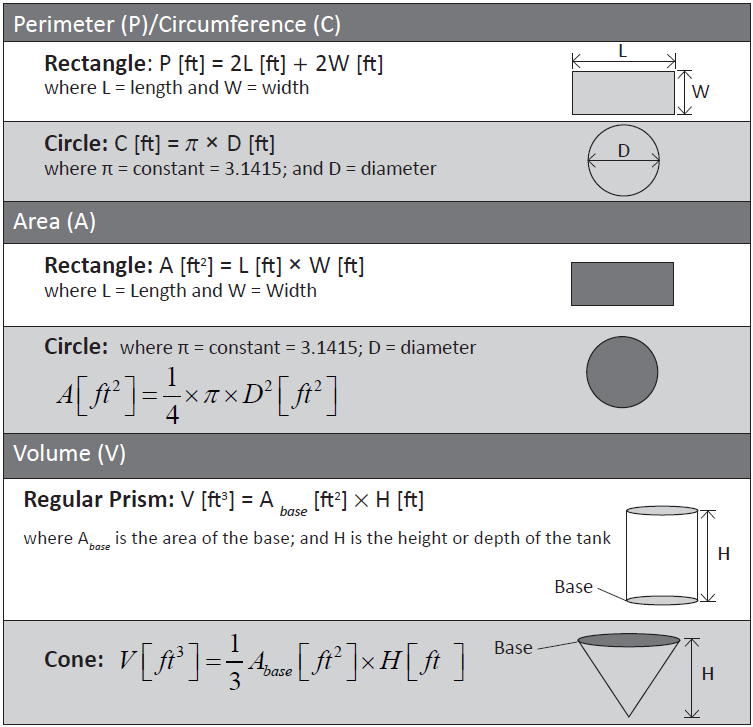
\includegraphics[scale=0.5]{Area&VolumeFormula}
\end{center}
\textbf{Example 1:} The floor of a rectangular building is 20 feet long by 12 feet wide and the inside walls are 10 feet high. Find the total surface area of the inside walls of this building\\
Solution:\\
% \begin{center}
\begin{tikzpicture}
	%%% Edit the following coordinate to change the shape of your
	%%% cuboid
      
	%% Vanishing points for perspective handling
	\coordinate (P1) at (-7cm,1.5cm); % left vanishing point (To pick)
	\coordinate (P2) at (8cm,1.5cm); % right vanishing point (To pick)

	%% (A1) and (A2) defines the 2 central points of the cuboid
	\coordinate (A1) at (0em,0cm); % central top point (To pick)
	\coordinate (A2) at (0em,-2cm); % central bottom point (To pick)

	%% (A3) to (A8) are computed given a unique parameter (or 2) .8
	% You can vary .8 from 0 to 1 to change perspective on left side
	\coordinate (A3) at ($(P1)!.8!(A2)$); % To pick for perspective 
	\coordinate (A4) at ($(P1)!.8!(A1)$);

	% You can vary .8 from 0 to 1 to change perspective on right side
	\coordinate (A7) at ($(P2)!.7!(A2)$);
	\coordinate (A8) at ($(P2)!.7!(A1)$);

	%% Automatically compute the last 2 points with intersections
	\coordinate (A5) at
	  (intersection cs: first line={(A8) -- (P1)},
			    second line={(A4) -- (P2)});
	\coordinate (A6) at
	  (intersection cs: first line={(A7) -- (P1)}, 
			    second line={(A3) -- (P2)});

	%%% Depending of what you want to display, you can comment/edit
	%%% the following lines

	%% Possibly draw back faces

	\fill[gray!40] (A2) -- (A3) -- (A6) -- (A7) -- cycle; % face 6
	\node at (barycentric cs:A2=1,A3=1,A6=1,A7=1) {\tiny Floor=W*L};
	
	\fill[gray!50] (A3) -- (A4) -- (A5) -- (A6) -- cycle; % face 3
	\node at (barycentric cs:A3=1,A4=1,A5=1,A6=1) {\tiny Wall - W*H};
	
	\fill[gray!10, opacity=0.2] (A5) -- (A6) -- (A7) -- (A8) -- cycle; % face 4
	\node at (barycentric cs:A5=1,A6=1,A7=1,A8=1) {\tiny Wall - L*H};
	
	\fill[gray!10,opacity=0.5] (A1) -- (A2) -- (A3) -- (A4) -- cycle; % f2
	\node at (barycentric cs:A1=1,A2=1,A3=1,A4=1) {\tiny Wall - L*H};
	
	\fill[gray!40,opacity=0.2] (A1) -- (A4) -- (A5) -- (A8) -- cycle; % f5
	\node at (barycentric cs:A1=1,A4=1,A5=1,A8=1) {\tiny Ceiling=W*L};	
	
	\draw[thick,dashed] (A5) -- (A6);
	\draw[thick,dashed] (A3) -- (A6);
	\draw[thick,dashed] (A7) -- (A6);

	%% Possibly draw front faces

	%\fill[orange] (A1) -- (A8) -- (A7) -- (A2) -- cycle; % face 1
	\node at (barycentric cs:A1=1,A8=1,A7=1,A2=1) {\tiny Wall - W*H};
	


	%% Possibly draw front lines
	\draw[thick] (A1) -- (A2);

	\draw[<->] (-1.8,0.38) -- (-1.8,-1.3)node [midway, above=-1.8mm] {\hspace{-1.3cm}\tiny Height=10'};
	\draw[<->] (-1.6,-1.4) -- (-.3,-2.1)node [midway, above=-2.6mm] {\hspace{-1.3cm}\tiny Length=20'};
	\draw[<->] (2.6,-1.13) -- (0.2,-2.2)node [midway, below=.6mm] {\hspace{1.2cm}\tiny Width=12'};
	\draw[thick] (A3) -- (A4);
	\draw[thick] (A7) -- (A8);
	\draw[thick] (A1) -- (A4);
	\draw[thick] (A1) -- (A8);
	\draw[thick] (A2) -- (A3);
	\draw[thick] (A2) -- (A7);
	\draw[thick] (A4) -- (A5);
	\draw[thick] (A8) -- (A5);
	
	% Possibly draw points
	% (it can help you understand the cuboid structure)
%	\foreach \i in {1,2,...,8}
%	{
%	  \draw[fill=black] (A\i) circle (0.15em)
%	    node[above right] {\tiny \i};
%	}
	% \draw[fill=black] (P1) circle (0.1em) node[below] {\tiny p1};
	% \draw[fill=black] (P2) circle (0.1em) node[below] {\tiny p2};
\end{tikzpicture}\\
% \end{center}
2 Walls W*H + 2 Walls L*H= $2*12*10ft^2 + 2*20*10ft^2$\\
$=240+400=\boxed{640ft^2}$\\

2 Walls W*H + 2 Walls L*H + Floor + Ceiling= $2*12*10ft^2 + 2*20*10ft^2 + 2*12*20ft^2$\\
$=240+400+480=\boxed{1,120ft^2}$\\

\textbf{Example 2:} How many gallons of paint will be required to paint the inside walls of a 40 ft long x 65 ft wide x 20 ft high tank if the paint coverage is 150 sq. ft per gallon.  Note:  We are painting walls only.  Disregard the floor and roof areas.\\
Solution:\\
\vspace{0.3cm}
% \begin{center}
\begin{tikzpicture}
	%%% Edit the following coordinate to change the shape of your
	%%% cuboid
      
	%% Vanishing points for perspective handling
	\coordinate (P1) at (-7cm,1.5cm); % left vanishing point (To pick)
	\coordinate (P2) at (8cm,1.5cm); % right vanishing point (To pick)

	%% (A1) and (A2) defines the 2 central points of the cuboid
	\coordinate (A1) at (0em,0cm); % central top point (To pick)
	\coordinate (A2) at (0em,-2cm); % central bottom point (To pick)

	%% (A3) to (A8) are computed given a unique parameter (or 2) .8
	% You can vary .8 from 0 to 1 to change perspective on left side
	\coordinate (A3) at ($(P1)!.8!(A2)$); % To pick for perspective 
	\coordinate (A4) at ($(P1)!.8!(A1)$);

	% You can vary .8 from 0 to 1 to change perspective on right side
	\coordinate (A7) at ($(P2)!.7!(A2)$);
	\coordinate (A8) at ($(P2)!.7!(A1)$);

	%% Automatically compute the last 2 points with intersections
	\coordinate (A5) at
	  (intersection cs: first line={(A8) -- (P1)},
			    second line={(A4) -- (P2)});
	\coordinate (A6) at
	  (intersection cs: first line={(A7) -- (P1)}, 
			    second line={(A3) -- (P2)});

	%%% Depending of what you want to display, you can comment/edit
	%%% the following lines

	%% Possibly draw back faces

	\fill[gray!40] (A2) -- (A3) -- (A6) -- (A7) -- cycle; % face 6
	\node at (barycentric cs:A2=1,A3=1,A6=1,A7=1) {};
	
	\fill[gray!50] (A3) -- (A4) -- (A5) -- (A6) -- cycle; % face 3
	\node at (barycentric cs:A3=1,A4=1,A5=1,A6=1) {\tiny Wall - W*H};
	
	\fill[gray!10, opacity=0.2] (A5) -- (A6) -- (A7) -- (A8) -- cycle; % face 4
	\node at (barycentric cs:A5=1,A6=1,A7=1,A8=1) {\tiny Wall - L*H};
	
	\fill[gray!10,opacity=0.5] (A1) -- (A2) -- (A3) -- (A4) -- cycle; % f2
	\node at (barycentric cs:A1=1,A2=1,A3=1,A4=1) {\tiny Wall - L*H};
	
	\fill[gray!40,opacity=0.2] (A1) -- (A4) -- (A5) -- (A8) -- cycle; % f5
	\node at (barycentric cs:A1=1,A4=1,A5=1,A8=1) {};	
	
	\draw[thick,dashed] (A5) -- (A6);
	\draw[thick,dashed] (A3) -- (A6);
	\draw[thick,dashed] (A7) -- (A6);

	%% Possibly draw front faces

	%\fill[orange] (A1) -- (A8) -- (A7) -- (A2) -- cycle; % face 1
	\node at (barycentric cs:A1=1,A8=1,A7=1,A2=1) {\tiny Wall - W*H};
	


	%% Possibly draw front lines
	\draw[thick] (A1) -- (A2);

	\draw[<->] (-1.8,0.38) -- (-1.8,-1.3)node [midway, above=-1.8mm] {\hspace{-1.3cm}\tiny Height=20'};
	\draw[<->] (-1.6,-1.4) -- (-.3,-2.1)node [midway, above=-2.6mm] {\hspace{-1.3cm}\tiny Length=40'};
	\draw[<->] (2.6,-1.13) -- (0.2,-2.2)node [midway, below=.6mm] {\hspace{1.2cm}\tiny Width=65'};
	\draw[thick] (A3) -- (A4);
	\draw[thick] (A7) -- (A8);
	\draw[thick] (A1) -- (A4);
	\draw[thick] (A1) -- (A8);
	\draw[thick] (A2) -- (A3);
	\draw[thick] (A2) -- (A7);
	\draw[thick] (A4) -- (A5);
	\draw[thick] (A8) -- (A5);
	
	% Possibly draw points
	% (it can help you understand the cuboid structure)
%	\foreach \i in {1,2,...,8}
%	{
%	  \draw[fill=black] (A\i) circle (0.15em)
%	    node[above right] {\tiny \i};
%	}
	% \draw[fill=black] (P1) circle (0.1em) node[below] {\tiny p1};
	% \draw[fill=black] (P2) circle (0.1em) node[below] {\tiny p2};
\end{tikzpicture}\\
% \end{center}
\vspace{0.3cm}
2 Walls W*H + 2 Walls L*H = $2*65*20ft^2 + 2*40*20ft^2= 2,600+1,600=4,200ft^2$\\
$\implies @150\dfrac{ft^2}{gal} \enspace paint \enspace coverage \enspace \rightarrow \enspace \dfrac{4,200\cancel{ft^2}}{150\dfrac{\cancel{ft^2}}{gal}}=\boxed{28 \enspace gallons}$
\vspace{0.3cm}
\textbf{Example 3:}  What is the circumference of a 100 ft diameter circular sedimentation tank?\\
\vspace{0.3cm}
Solution:\\
\vspace{0.3cm}
$Circumference=\pi*D=3.14*100ft=\boxed{314ft}$
\vspace{0.3cm}

\textbf{Example 4:} If the surface area of a clarifier is 5,025$ft^2$, what is its diameter?\\
\vspace{0.3cm}
Solution:\\
\vspace{0.3cm}
$Surface \enspace area=\dfrac{\pi}{4}*D^2 \enspace \implies 5025(ft^2)=0.785*D^2 (ft^2)$\\
$\implies D^2=\dfrac{5025}{0.785} \implies D=\sqrt{6401.3}=\boxed{80ft}$
\vspace{0.3cm}

\textbf{Example 5:} How many gallons of water would 600 feet of 6-inch diameter pipe hold, approximately?\\
\vspace{0.3cm}
Solution:\\

\vspace{0.3cm}
% \begin{center}
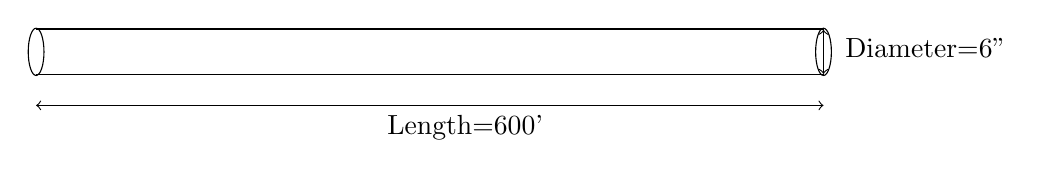
\begin{tikzpicture}
\draw (0,0) ellipse (0.1cm and 0.3cm);
\draw (10,0) ellipse (0.1cm and 0.3cm);
\draw [-] (0,-0.29) -- (10,-0.29);
\draw [-] (0,0.29) -- (10,0.29);
\draw [<->] (10,-0.28) -- (10,0.28) node [midway, below=-3mm] {\hspace{2.6cm}Diameter=6"};
\draw [<->] (0,-.68) -- (10,-.68)node [midway, below] {\hspace{0.9cm}Length=600'};
\end{tikzpicture}
% \end{center}
\vspace{0.3cm}
$Volume=\dfrac{\pi}{4}D^2*L=0.785*\Big(\dfrac{6}{12}\Big)^2*600\cancel{ft^3}*7.48\dfrac{gallons}{\cancel{ft^3}}=\boxed{881 \enspace gallons}$


\section{Flow and Velocity}\index{Flow and Velocity}
\begin{itemize}
\item Flow Rate - Q (volume/time) = velocity (distance or length traveled /time) * surface area
\item Velocity is the speed at which the water is flowing.  It is measured in units of length/time – ft./sec.
\item Velocity of water flowing through can be calculated by dividing the flow rate by area of the flow stream.\\
\vspace{0.5cm}
$$Velocity \enspace \dfrac{length}{time}= \dfrac{flow \enspace rate(\dfrac{volume \enspace or \enspace cubic \enspace length}{time})}{surface \enspace area \enspace in \enspace the \enspace direction \enspace of \enspace flow-square \enspace length}$$
\vspace{0.5cm}
\textbf{For a flow in a channel:}\\
\vspace{0.5cm}
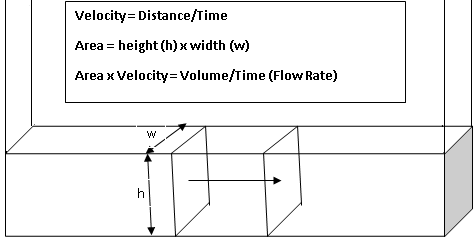
\includegraphics[scale=0.5]{ChannelFlow3}\\

\textbf{For a flow in a pipe:}\\
\vspace{0.5cm}
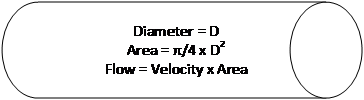
\includegraphics[scale=0.65]{VelocityinPipe}\\
\vspace{0.5cm}
\end{itemize}

\textbf{Example 1:} If a chemical is added in a pipe where water is flowing at a velocity of 3.1 feet per second, how many minutes would it take for the chemical to reach a point 7 miles away?  \\

Note - we want the answer in minutes\\

$$\textrm{Min } = \dfrac{1}{3.1}\dfrac{sec}{ft}*\dfrac{5280ft}{mile}*7 miles*\dfrac{min}{60 sec} = \boxed{199 min}$$
\\

\textbf{Example 2:} Find the flow in cfs in a 6 -inch line, if the velocity is 2 feet per second.

\begin{enumerate}
\item Determine the cross-sectional area of the line in square feet. Start by converting the diameter of the pipe to inches.

The diameter is 6 inches: therefore, the radius is 3 inches. 3 inches is $3 / 12$ of a foot or $0.25$ feet.

\item Now find the area in square feet.
$$
\begin{aligned}
&A=\pi \times r^{2} \\
&A=\pi \times\left(0.25 \mathrm{ft}^{2}\right. \\
&A=\pi \times 0.0625 \mathrm{ft}^{2} \\
&A=0.196 \mathrm{ft}^{2}
\end{aligned}
$$
Or
$$
\begin{aligned}
&A=0.785 \times D^{2} \\
&A=0.785 \times 0.5^{2} \\
&A=0.785 \times .05 \times .05 \\
&A=0.196 \mathrm{ft}^{2}
\end{aligned}
$$

\item Now find the flow.

$\mathrm{Q}=\mathrm{V} \times \mathrm{A}$

$\mathrm{Q}=2 \mathrm{ft} / \mathrm{sec} \times 0.196 \mathrm{ft}^{2}$

$\mathrm{Q}=0.3927 \mathrm{cfs}$ or $0.4 \mathrm{cfs}$
\end{enumerate}



\section{Unit Conversions}\index{Unit Conversions}
\begin{itemize}
\item A conversion is a number that is used to multiply or divide into a measure in order to change the units of the original measure.

\begin{table}[h!]

\begin{center}
    \begin{tabular}{ | p{4cm} |p{8cm}|}
    \hline
    
\textbf{Measure} & \textbf{Units}\\
\hline   
Length  & inches, ft, miles\\
\hline 
Area  & ft$^2$, acres \\
\hline 
Volume & ft$^3$, gallons, acres-ft.\\
\hline 
Density & weight per volume, lbs/ft$^3$, lbs/gallon\\
\hline 
Flow & ft$^3$/min, MGD, acres-ft/day\\
\hline 

	

    \end{tabular}
 \caption{Common units in water calculations}	
    \end{center}

    \end{table}

\item In most instances, the conversion factor cannot be derived. It must be known. Therefore, tables such as the one below are used to find the common conversions.\\
\begin{tabular}{|l|l|}
\hline
Some Common Conversions & Weight \\
\hline
Linear Measurements & $1 \mathrm{ft}^{3}$ of water $=62.4 \mathrm{lbs}$ \\
\hline
1 inch $=2.54 \mathrm{~cm}$ & $1 \mathrm{gal}=8.34 \mathrm{lbs}$ \\
$1 \mathrm{foot}=30.5 \mathrm{~cm}$ & $1 \mathrm{lb}=453.6 \mathrm{grams}$ \\
$1 \mathrm{~meter}=100 \mathrm{~cm}=3.281 \mathrm{feet}=39.4$ inches 1 & $1 \mathrm{~kg}=1000 \mathrm{~g}=2.2 \mathrm{lbs}$ \\
acre $=43,560 \mathrm{ft}^{2}$ & $1 \%=10,000 \mathrm{mg} / \mathrm{L}$ \\
$1 \mathrm{yard}=3 \mathrm{feet}$ & $1 \mathrm{pound}=16 \mathrm{oz} \mathrm{dry} \mathrm{wt}$ \\
 & $1 \mathrm{ft}^{3}=62.4 \mathrm{lbs}$ \\
\hline
Volume & Pressure \\
\hline
$1 \mathrm{gal}=3.78$ liters & $1 \mathrm{ft}$ of head $=0.433 \mathrm{psi}$ \\
$1 \mathrm{ft}=7.48$ gal & $1 \mathrm{psi}=2.31 \mathrm{ft}$ of head \\
$1 \mathrm{~L}=1000 \mathrm{~mL}$ &  \\
$1 \mathrm{gal}=16 \mathrm{cups}$ &  \\
\hline
Flow &  \\
\hline
$1 \mathrm{cfs}=448 \mathrm{gpm}$ &  \\
$1 \mathrm{gpm}=1440 \mathrm{gpd}$ &  \\
\hline
\end{tabular}
\vspace{0.2cm}
\item Common conversions in water related calculations include the following:

\begin{itemize}
  \item gpm to cfs

  \item Million gallons to acre feet

  \item Cubic feet to acre feet

  \item Cubic feet of water to gallons


  \item gpm to MGD 

  \item psi to feet of head

\end{itemize}

\item Steps for unit conversion:\\
\begin{enumerate}[Step 1:]
\item \texthl{Make sure the original unit is for the same measurement as the converted (desired) unit.}  So if the original unit is for area, say in ft$^2$ the converted unit should be another area unit such as in$^2$ or acre but it cannot be gallons as gallon is a unit of volume.\\
Note:  Calculating the weight of a certain volume of water involves the use of density which is the mass per volume -  value in units including lbs/gallon or lbs/$ft^3$\\

\item Write down the conversion formula as:\\

$Quantity \enspace in \enspace converted \enspace unit = Quantity \enspace (\cancel{Original \enspace Unit}) *   Conversion  \enspace Factor \enspace  \dfrac{Conversion \enspace unit}{\cancel{Original \enspace unit}}$\\
\end{enumerate}

\item Note:  If you wish to convert cubic feet of water to pounds, you have to use its density which is the known mass per unit volume.\\
$\dfrac{8.34 \enspace lbs}{gallon}$ or $\dfrac{62.4 \enspace lbs}{ft^3}$\\
$mass \enspace of \enspace water = \cancel{Volume} *   Density  (\dfrac{mass}{\cancel{Volume}})$\\

\end{itemize}

Example Problems:\\
\begin{enumerate}
\item Convert 1000 $ft^3$ to cu. yards\\

$1000 \cancel{ft^3}*\dfrac{cu.yards}{27\cancel{ft^3}} = 37 cu.yards$

\item Convert 10 gallons/min to $ft^3$/hr\\
Note:  This involves use of two conversion factors - one for converting gallons to cubic feet and another for converting minute to gallons.\\ 
$\dfrac{10 \cancel{gallons}}{\cancel{min}}*  \dfrac{ft^3}{7.48 \cancel{gallons}}  * \dfrac{60 \cancel{min}}{hr}   = \dfrac{80.2ft^3}{hr}$


\item Convert 100,000 $ft^3$ to acre-ft.\\
$100,000 \cancel{ft^3} * \dfrac{acre-ft}{43,560 \cancel{ft^2-ft}} =  2.3 acre-ft$\\

\item Convert 8 $ft^3$ of water to pounds.\\
Here the conversion is from a volume ($ft^3$) to a weight (lbs).  It involves use of a standard correlation of the volume of water to its weight - its density. 

$Weight \enspace of \enspace water \enspace in \enspace lbs=8 \cancel{ft^3} *   62.4  (\dfrac{lbs}{\cancel{ft^3}}) = 499.2 \enspace lbs $\\

\end{enumerate}

\subsection{Temperature Conversion}\index{Temperature Conversion}
\begin{itemize}
\item Two scales are commonly used to measure temperature: degrees Fahrenheit (\degree{F}) and degrees Centigrade or Celsius(\degree{C}). 
\item Fahrenheit is the standard scale used in the U.S. and Celsius is the metric scale. 
\item In the Celsius scale, water freezes at 0\degree{C} and boils at 100\degree{C}. In the Fahrenheit scale, water freezes at32\degree{F} and boils at 212\degree{F}. 
\item The following factors can be used when converting from one temperature scale to another:
$$\degree{C} = \dfrac{\degree{F}-32}{1.8}$$

$$\degree{F}=(\degree{C} \times 1.8)+32$$
\end{itemize}


\section{Concentration}\index{Concentration}
\begin{itemize}
\item Concentration is typically expressed as mg/l which is the weight of the constituent (mg) in 1 liter of water.
\item As 1 liter of water weighs 1 million mg, a concentration of 1 mg/l implies 1 mg of constituent per 1 million mg of water or one part per million (ppm).   \texthl{Thus, mg/l and ppm are synonymous.}
\item Sometimes the constituent concentration is expressed in terms of percentage.\\
\vspace{6pt}
\textbf{Example:} 12.5\% chlorine concentration solution.\\
\vspace{0.2cm}
100\% would mean 1,000,000 mg/l or 1,000,000 ppm\\
\vspace{0.2cm}
$\implies$1\% would be $\dfrac{1,000,000}{100}\textrm{mg/l} = \textrm{10,000 mg/l or 10,000 ppm}$\\
\vspace{0.2cm}
$\implies$12.5\% chlorine concentration is 125,000 mg/l or 125,000 ppm.
\vspace{6pt}

$1\% \enspace concentration = 10,000 \enspace ppm \enspace or \enspace\dfrac{mg}{l}$\\
$0.1\% \enspace concentration = 1,000 \enspace ppm \enspace or \enspace \dfrac{mg}{l}$\\
$0.01\% \enspace concentration = 100 \enspace ppm \enspace or \enspace \dfrac{mg}{l}$\\
$10\% \enspace concentration = 100,000 \enspace ppm \enspace or \enspace \dfrac{mg}{l}$\\
$5\% \enspace concentration = 50,000 \enspace ppm \enspace or \enspace \dfrac{mg}{l}$\\
$12.5\% \enspace concentration = 125,000 \enspace ppm \enspace or \enspace \dfrac{mg}{l}$\\
\end{itemize}

\vspace{0.3cm}
Above concepts are used for chemicals such as fluoride and hypochlorites - the strength of the product as used is commonly expressed as a percentage.
\vspace{0.3cm}

\textbf{Example 1:} A chlorine solution was made to have a $4 \%$ concentration. It is often desirable to determine this concentration in $\mathrm{mg} / \mathrm{L}$. This is relatively simple: the $4 \%$ is four percent of a million.

To find the concentration in $\mathrm{mg} / \mathrm{L}$ when it is expressed in percent, do the following:

\begin{enumerate}
  \item Change the percent to a decimal.
\end{enumerate}
$$
4 \% \div 100=0.04
$$

\begin{enumerate}
  \setcounter{enumi}{2}
  \item Multiply times a million.
\end{enumerate}
$$
0.04 \times 1,000,000=40,000 \mathrm{mg} / \mathrm{L}
$$
We get the million because a liter of water weighs $1,000,000 \mathrm{mg} .1 \mathrm{mg}$ in 1 liter is 1 part in a million parts ( $\mathrm{ppm}) .1 \%=10,000 \mathrm{mg} / \mathrm{L}$.


\textbf{Example 2:} How much $65 \%$ calcium hypochlorite is required to obtain 7 pounds of pure chlorine?\\
$65 \%$ implies that in every lb of calcium hypochlorite has $65 \%$ lbs of available chlorine.\\
\vspace{0.2cm}
Therefore, $\dfrac{0.65 \textrm{ lbs available chlorine}}{\textrm{lb of calcium hypochlorite}} $ or conversely $\dfrac{\textrm{lb of calcium hypochlorite}}{0.65 \textrm{ lbs available chlorine}}$\\
\vspace{0.2cm}
$\implies{\textrm{lbs calcium hypchlorite required}}=\dfrac{\textrm{lb of calcium hypochlorite}}{0.65 \cancel{\textrm{ lbs available chlorine}}}*\dfrac{7\cancel{\textrm{ lb of available chlorine}}}{}$\\
\vspace{0.2cm}
$=\boxed{10.8 \textrm{ lbs of calcium hypochlorite with } 65\%\textrm{available chlorine is required}}$

\section{Density}\index{Density}
\begin{itemize}
\item Density is defined as the weight of a substance per a unit of its volume. For example, pounds per cubic foot or pounds per gallon.

\item Here are a few key facts about density:
\begin{itemize}

\item Density is measured in units of lb/ft3, lb/gal, or mg/L. Density of water = 62.4 lb/ft3 = 8.34 lb/gal.
\end{itemize}
\end{itemize}

\section{Specific Gravity}\index{Specific Gravity}
\begin{itemize}
\item Specific gravity is the ratio of the density of a substance (liquid or solid) to the density water.
\item It is the ratio of the weight of the substance of a certain volume to the weight of water of the same volume.

\item Any substance with a density greater than that of water will have a specific gravity greater than 1.0. Any substance with a density less than that of water will have a specific gravity less than 1.0. 

\item Specific gravity examples:
\begin{itemize}

\item Specific gravity of water = 1.0 
\item Specific gravity of concrete = 2.5 (depending on ingredients)
\item Specific gravity of alum (liquid @ 60°F) = 1.33 
\item Specific gravity of hydrogen peroxide (35\%) = 1.132
\end{itemize}

\item Specific gravity is used in two ways:
\begin{enumerate}
\item To calculate the total weight of a \% solution (either as a single gallon or a drum volume).\\
Total Weight = Drum Vol X SG X 8.34
\item To calculate the “active ingredient” weight of a single gallon or a drum.\\

Active Ingredient Weight within Drum = Drum Volume X SG X 8.34 X \% solution as a decimal. (i.e., Total Weight X \% solution as a decimal)\\

NOTE: Both ways start with solving for the total weight (Drum Vol X SG X 8.34). When solving for “active ingredient” weight, you have to then multiply by \% solution as a decimal.

\end{enumerate}
\end{itemize}

\textbf{Example:} What is the weight of 5 gallons of a 40\% ferric chloride solution given its specific gravity of 1.43?
$$(8.34 * 1.43) \enspace lbs/gal*5 \enspace gallons = \boxed{59.6 \enspace lbs}$$

The weight of active ferric chloride in the drum will be 59.6*0.4=23.84 lbs (as ferric chloride is 40\% strength)

\section{Contaminant Removal Efficiency}\index{Contaminant Removal Efficiency}
\begin{itemize}
\item Contaminant removal efficiency can be expressed as the percentage of the inlet concentration removed and can be established based upon the amount of a particular contaminant entering and leaving a treatment process.

\item $Percent \enspace Removal \enspace (\%) = \dfrac{Concentration \enspace  In-Concentration\enspace  Out}{Concentration \enspace In}*100$\\

\item If 10 units of a contaminant are entering a process and 8 units of pollutant are leaving (process removes 2 units), then the process removal rate for that pollutant is (10-8)/10*100=20\%.  In this example the process is 20\% efficient in removing that particular contaminant.

\item Besides percent removal, removal efficiency can also be expressed in terms of Log removal.
\item Background of log:\\ 
Log of a number $x$ to the \textbf{base} $B$ is the exponent to which $B$ must be \textbf{raised} to produce $x$.\\
\vspace{0.3cm}
\begin{center}
$\log_B x=A \implies B^A=x$\\
For Example: $\log_{10} 1000=3 \implies 10^3=1000$ \\
\end{center}
\vspace{0.3cm}
Log Rules\\
\begin{enumerate}
\item $\log_{b} 1=0$
\item $\log_{b} ac=\log_{b} a + \log_{b} c$
\item $\log_{b} \dfrac{a}{c}=\log_{a} a - \log_{b} c$
\item $\log_{b} a^r=r\log_{b} a$
\item $\log_{b} \dfrac{1}{c}=-\log_{b} c$
\end{enumerate}
\vspace{0.3cm}
\item Log removal is:  $\log_{10} {(Concentration \enspace In)} - \log_{10} {(Concentration \enspace Out)}$
\item \textbf{CASE 1: } Say the initial (before treatment) and final (after treatment) cryptosporidium concentrations are 100 oocysts and 10 oocysts per L respectively. \\
\vspace{0.3cm}
Thus log removal is $\log_{10} 100 - \log_{10} 10 = \log_{10}\dfrac{100}{10}=\log_{10} 10 = \boxed{1} \enspace as \enspace 10^1=10 $\\
\vspace{0.3cm}
\item The removal on a percentage basis: $\mathrm{Percent \enspace removal} = \dfrac{\mathrm{initial}-\mathrm{final}}{\mathrm{intial}}*100=\dfrac{100-10}{100}*100=90\%$\\
\item \textbf{CASE 2: } Say the initial (before treatment) and final (after treatment) cryptosporidium concentrations are 100 oocysts and 1 oocysts per L respectively. \\
\vspace{0.3cm}
Thus log removal is $\log_{10} 100 - \log_{10} 1 = \log_{10}\dfrac{100}{1}=\log_{10} 100 = \boxed{2} \enspace as \enspace 10^2=100 $\\
\vspace{0.3cm}
\item The removal on a percentage basis: $\mathrm{Percent \enspace removal} = \dfrac{\mathrm{initial}-\mathrm{final}}{\mathrm{intial}}*100=\dfrac{100-1}{100}*100=99\%$\\
\vspace{0.5cm}
\item \textbf{CASE 3: } If the initial (before treatment) and final (after treatment) cryptosporidium concentrations are 1000 oocysts and 1 oocysts per L respectively. (unreal values....) \\
\vspace{0.3cm}
Thus log removal is $\log_{10} 1000 - \log_{10} 10 = \log_{10}\dfrac{1000}{1}=\log_{10} 1000 = \boxed{3} \enspace as \enspace 10^3=1000 $\\
\vspace{0.3cm}
The removal on a percentage basis: $\mathrm{Percent \enspace removal} = \dfrac{\mathrm{initial}-\mathrm{final}}{\mathrm{intial}}*100=\dfrac{1000-1}{1000}*100=99.9\%$
\vspace{0.3cm}
\item Thus:\\
1 log removal =90\% removal efficiency\\
2 log removal =99\% removal efficiency\\
3 log removal =99.9\% removal efficiency\\
4 log removal =99.99\% removal efficnecy\\
\end{itemize}

\section{Pounds Formula}\index{Pounds Formula}
\begin{itemize}
\item Pounds formula: 
$$lbs \enspace \textbf{or} \enspace \dfrac{lbs}{day}=Concentration\Big(\dfrac{mg}{l}\Big)*8.34*volume(MG) \enspace \textbf{or} \enspace Flow (MGD)$$\\
\item So if the concentration of a particular constituent (in mg/liter) and the volume or flow of wastewater is given, one can calculate the amount of that constituent or using this formula.\\
\texthl{Important notes:}\\
\begin{enumerate}
\item \texthl{The unit of the constituent loading rate will be in lbs per the unit of time the flow is expressed in.  So if the flow is in MG per day the calculated loading rate will be in lbs/day.  Likewise if the flow value used is in MG per minute, the calculated loading rate will be in lbs/min.}
\item \texthl{If volume is used, the calculated value will be the mass of the constituent in that volume.  If flow is used, the calculated value will be the mass of the constituent in that flow.}
\item \texthl{For the Pound Formula to work, the volume or flow needs to be expressed in MG.  Volume or flows in other units - gallons, $ft^3$ etc. needs to be converted to MG.}
\end{enumerate}

\item The formula assumes that all of the material found in water (TSS, BOD, MLSS, Chlorine, etc.) weighs the same as water, that is, $8.34$ pounds per gallon.
\item In the Pounds Formula, there are three variables – lbs, concentration and volume, and one constant - 8.34.  Knowing any of the two variables in the formula, one can calculate the third (unknown) variable by rearranging the equation.\\
\begin{figure}[h]
\begin{tikzpicture}
    \newcommand{\R}{3}

\path[help lines,step=.2] (0,0) grid (16,6);
\path[help lines,line width=.6pt,step=1] (0,0) grid (16,6);
%\foreach \x in {0,1,2,3,4,5,6,7,8,9,10,11,12,13,14,15,16}
%\node[anchor=north] at (\x,0) {\x};
%\foreach \y in {0,1,2,3,4,5,6}
%\node[anchor=east] at (0,\y) {\y};
%-------------CIRCLE-----------------------------------
\draw[black,fill=gray!10] (8,3) circle (\R);
\draw[black, very thick, rotate=0](5,3) -- (11,3);
\draw (8,4.5) node[text width=3cm,align=center]
  {\scriptsize{lbs or lbs/day}};
\draw (6.4,2) node[text width=3cm,align=center]
  {\scriptsize{Concentration\\mg/l}};
\draw (9.7,2) node[text width=3cm,align=center]
  {\scriptsize{Volume(MG)\\Flow(MGD)}};
  \draw (8,1)node[text width=3cm,align=center]
  {\scriptsize{8.34}};
\draw[black, very thick, rotate=0](6.4,0.5) -- (8,3);
\draw[black, very thick, rotate=0](9.6,0.5) -- (8,3);
  \node [circle split,draw,double,fill=red!20] at (4,3)
  {
    % No \nodepart has been used, yet. So, the following is put in the
    % ``text'' node part by default.
    $\div$
    \nodepart{lower} % Ok, end ``text'' part, start ``output'' part
    $=$
  };
  
    \node [circle split,draw,double,fill=red!20] at (5.8,-0.2)
  {
    % No \nodepart has been used, yet. So, the following is put in the
    % ``text'' node part by default.
    \scriptsize{$X$}
    \nodepart{lower} % Ok, end ``text'' part, start ``output'' part
    \tiny{$Multiply$}
  };
  
    \node [circle split,draw,double,fill=red!20] at (10,-0.2)
  {
    % No \nodepart has been used, yet. So, the following is put in the
    % ``text'' node part by default.
    \scriptsize{$X$}
    \nodepart{lower} % Ok, end ``text'' part, start ``output'' part
    \tiny{$Multiply$}
  };
\end{tikzpicture}
\caption{Davidson Pie}
\end{figure}
\vspace{0.2cm}
\item Davidson Pie provides a pictorial reference for calculating any unknown variable.  If for example, if Concentration is unknown, it can be calculated as follows: \\$$Concentration\Big(\dfrac{mg}{l}\Big)=\dfrac{lbs \enspace \textbf{or} \enspace \dfrac{lbs}{day}}{8.34*Volume(MG) \enspace \textbf{or} \enspace Flow (MGD)}$$\\
\vspace{0.2cm}
\item Likewise, if Volume (or Flow) is the unknown variable. it can be calculated as:  \\$$Volume (MG) \enspace or \enspace Flow(MGD)=\dfrac{lbs \enspace \textbf{or} \enspace \dfrac{lbs}{day}}{Concentration\Big(\dfrac{mg}{l}\Big)* \enspace 8.34  }$$
\vspace{0.2cm}
\item Pounds formula is used for:
\begin{itemize}
\item Calculating the quantity in pounds of a particular wastewater constituent entering or leaving a wastewater treatment process
\item Calculating the pounds of chemicals to be added\\
\end{itemize}
\end{itemize}


\textbf{Example 1:} If a 5 MGD flow is to be dosed with 25 mg/l of a certain chemical, calculate the lbs/day that chemical required.\\

Solution\\

Applying lbs formula:\\
$\dfrac{lbs}{day}=5 MGD *250\dfrac{mg}{l}*8.34 = \boxed{1,042\dfrac{lbs}{day}}$
\\
\vspace{6pt}
\textbf{Example 2:} Calculate the lbs of chemical in 7,500 gallons of 4.5\% active solution of that chemical.\\
Solution\\
Applying lbs formula:\\
$lbs chemical = \dfrac{7500}{1,000,000}MG * 4.5*10,000 *8.34 = \boxed{2,815 \enspace lbs \enspace chemical}$\\
\textbf{Note:}\\  
1) 7500 gallons was converted to MG by dividing by 1,000,000\\
$7500 \enspace gallons * \dfrac{1 MG}{1,000,000 \enspace gallon}$\\
2) 4.5\% was converted to mg/l by multiplying by 10,000 as 1\%=10,000mg/l


\section{Chemicals Related Math Problems}\index{Chemicals Related Math Problems}
\subsection{Chemical Dosing}\index{Chemical Dosing}

\begin{itemize}
\item Use lbs formula to calculate the lbs of chemicals required\\
\item Using the calculated lbs chemical required value, calculate the amount of that chemical at the concentration available
\end{itemize}

\textbf{Example 1:} If a 5 MGD flow is to be dosed with 25 mg/l of a certain chemical, calculate the lbs/day that chemical required.\\

Solution\\

Applying lbs formula:\\
$\dfrac{lbs}{day}=5 MGD *250\dfrac{mg}{l}*8.34 = \boxed{1,042\dfrac{lbs}{day}}$
\\
\vspace{6pt}
\textbf{Example 2:} Calculate the lbs of chemical in 7,500 gallons of 4.5\% active solution of that chemical.\\
Solution\\
Applying lbs formula:\\
$lbs chemical = \dfrac{7500}{1,000,000}MG * 4.5*10,000 *8.34 = \boxed{2,815 \enspace lbs \enspace chemical}$\\


\textbf{Example 3:} How many gallons per day of bleach solution (SG 1.2)containing 12.5\% available chlorine is required to disinfect a 10 MGD flow of water given the required chlorine dosage of 7 mg/l.\\
\begin{enumerate}
\item Calculate the lbs of chlorine required using the lbs formula:\\
\vspace{0.5cm}
=$10 MGD \enspace * \enspace 7 \dfrac{mg}{l} \enspace * \enspace 8.34\enspace=\enspace 583.8 \enspace lbs \enspace chlorine \enspace per \enspace day$\\
\vspace{0.5cm}
\item Calculate the gallons of bleach which will provide the 583.8 lbs chlorine\\
\vspace{0.5cm}
Applying the lbs formula - note that 8.34 * SG will give the actual lbs/gal of bleach.  If SG is not provided, use only 8.34 lbs per gallon:\\
\vspace{0.5cm}
$583.8 \dfrac{lbs \enspace bleach}{day}\enspace=\enspace x \dfrac{gal}{day} \enspace * \enspace 8.34 * 1.2 \dfrac{lbs \enspace bleach}{gal} \enspace * \enspace 0.0125 \dfrac{lbs \enspace chlorine}{lb \enspace bleach} \enspace $\\
\vspace{0.5cm}
$ \implies x \dfrac{gal}{day}\enspace = \enspace \dfrac{583.8}{8.34*1.2*0.125} \enspace = \boxed{467 \dfrac{gal}{day}}$
\end{enumerate}
\vspace{0.3cm}
\textbf{The above problem can be solved directly using the formula below given in the SWRCB Water Treatment Exam Formula Sheet.}\\
\vspace{0.3cm}
 $\textrm{GPD}=\dfrac{\textrm{(MGD)}*\textrm{(ppm or mg/l)}*8.34 \enspace \textrm{lbs/gal}}{\textrm{\% \enspace purity}*\textrm{Chemical \enspace Wt. (lbs/gal)}}$ 
 \vspace{0.3cm}
 $\textrm{GPD}=\dfrac{10*7*8.34}{0.125*(1.2*8.34)}=\boxed{467 \dfrac{\textrm{gal}}{\textrm{day}}}$ 


\subsection{Blending and Dilution Calculations}\index{Blending and Dilution Calculations}
\begin{itemize}
\item Blending and dilution calculations apply to the following scenarios:
\begin{itemize}
\item Blending involves mixing two streams - each with a different concentration of contaminant/chemical, to obtain a certain volume or flow containing the target concentration of contaminant/chemical.  For example: \textit{Finding the correct blend of two source water streams - one with 15 mg/L of iron and other containing  4 mg/L of iron to get a 100 gpm product water containing 8 mg/l of iron.} \textbf{OR}\\
\textit{Calculating the actual combined TDS concentration obtained by mixing two known flows with known TDS concentrations.}
\item Dilution involves makedown of a higher concentration of a chemical to a lower concentration using water as a dilutant.   For example: \textit{How much initial volume of a 4\% polymer solution is needed to make 3500 gallons of polymer at 0.25\% concentration?}\\
\end{itemize}
\item These type of problems are solved using C*V relationship where:
\begin{itemize}
 \item C is the concentration expressed in ppm or mg/l or as \% purity.
 \item V is either the volume or flow.
\item The product - C*V - $\dfrac{\textrm{\textrm{mass}}}{\textrm{volume}/\textrm{flow}}*\textrm{volume/flow} = \textrm{mass}$  
\end{itemize}
\item For blended streams, the sum of the mass from each of the two source streams will equal to the mass in the target stream:

\item Thus, \textbf{for blending calculations}, if:\\

C$_1$ and V$_1$ is the concentration and volume respectively of the one of the sources streams and\\
\vspace{0.2cm}
 C$_2$ and V$_2$ is the concentration and volume respectively of the second source stream, and \\
 \vspace{0.2cm}
C$_3$ and and V$_3$ is the concentration and volume respectively of the target stream\\
\vspace{0.3cm}
The sum of the mass from each of the two source streams will equal to the mass in the target stream:\\
\vspace{0.3cm}
\textbf{C$_1$ * V$_1$ + C$_2$ * V$_2$ =  C$_3$ * V$_3$.}\\
\vspace{0.3cm}
This equation can be manipulated algebraically to calculate anyone of the unknown values in the equation.\\
\vspace{0.2cm}
Also, any of the three volume variables can be expressed as the sum or difference of the other two - , or V$_1$ + V$_2$ = V$_3$ or V$_1$ = V$_3$ - V$_2$ or V$_2$ = V$_T$ - V$_1$\\

\item \textbf{For dilution}, the mass of the target chemical will remain the same, as only water is added to the source (concentrated chemical).
\item Thus, for dilution calculations, if:\\
\vspace{0.2cm}
C$_1$ and V$_1$ is the concentration and volume respectively of the concentrated product used for the dilution, and\\
\vspace{0.2cm}
C$_2$ and V$_2$ is the concentration and volume of the resultant product after dilution with water\\
\vspace{0.2cm}
The mass of the target chemical in the volume of the concentrated product used for dilution will remain the same in the final diluted product:\\
\vspace{0.3cm}
\textbf{C$_1$ * V$_1$ =  C$_2$ * V$_2$.}\\

\end{itemize}

\textbf{Example Problem \#1:} Two wells are used to satisfy demand during the summer months. One well produces water that contains 22 mg/L of Arsenic. The other well produces water that contains 3 mg/L of Arsenic. If the total demand for water is 400 gpm and the target Arsenic concentration in the finished water is 8 mg/L, what is the highest pumping rate possible for the first well?\\
\vspace{0.3cm}
\textbf{Solution:}\\
C$_1$ * V$_1$ + C$_2$ * V$_2$ =  C$_3$ * V$_3$\\
\vspace{0.3cm}
Thus 22 * V$_{22}$ + 3 * V$_3$ =  8 * V$_8$\\
\vspace{0.3cm}

V$_{22}$ + V$_3$ = V$_8$ = 400 gpm\\
\vspace{0.3cm}
As we want to solve for V$_{22}$, we can express V$_3$ as: V$_3$ = 400-V$_{22}$\\
\vspace{0.3cm}
Thus, 22 * V$_{22}$ + 3 * (400-V$_{22}$) =  8 * 400=3,200\\
\vspace{0.3cm}
22V$_{22}$ + 1200-3V$_{22}$ =  3,200\\
\vspace{0.3cm}
V$_{22}$(22-3) =  2,000\\
\vspace{0.3cm}
V$_{22}$ = $ \dfrac{2,000}{19}=\boxed{105.3 \enspace gpm}$\\
\vspace{0.3cm}
Also, V$_3$=400-105.3=294.7\\
\vspace{0.3cm}

NOTE:  If one does not want to utilize algebraic manipulation, one may memorize the following formula:\\
\vspace{0.3cm}
$V_{1/2}=\dfrac{\lvert C_3 - C_{2/1}\rvert*V_3}{C_1-C_2}$\\
\vspace{0.3cm}
Applying the formula above to Example Problem \#2:\\
\vspace{0.3cm}
$V_{22}=\dfrac{\lvert 8 - 3\rvert*400}{22-3}=\boxed{105.3 \enspace gpm}$\\
\vspace{0.3cm}
$V_{3}=\dfrac{\lvert 8 - 22\rvert*400}{22-3}=\boxed{294.7 \enspace gpm}$\\
\vspace{0.3cm}
\textbf{Example Problem \#2:}  How many gallons of a 4\% polymer solution is required to make a 3,500 gallon batch of 0.25\% polymer solution.\\

\textbf{Solution:}\\
\vspace{0.3cm}
Here, we are adding water - which has zero percent of polymer concentration to the 4\% polymer to make a 0.25\% polymer solution.\\
\vspace{0.3cm}
C$_1$ * V$_1$ = C$_2$ * V$_2$\\
\vspace{0.3cm}
C$_{4\%}$ * V$_{4\%}$ =  C$_{0.25\%}$ * V$_{0.25\%}$\\
\vspace{0.3cm}
4 * V$_{4\%}$ =  0.25 * 3,500\\
\vspace{0.3cm}
$\implies V_{4\%} = \dfrac{0.25 \enspace * \enspace 3500}{4}= \boxed{219 \enspace\textrm{gal}} $\\
\vspace{0.3cm}
Take 219 gallons of the 4\% polymer and dilute to 3,500 gallons to give a 0.25\% polymer solution.\\


%\section{Unaccounted water}\index{unaccounted water calculation}
%
%Consumption—refers to actual (metered) or estimated water uses within a distribution network. Consumption includes metered or estimated customer usage and can also include authorized uses that can be estimated such as firefighting, main flushing, and street cleaning.\\
%Unaccounted-for Water is the difference between the amount of water produced and the amount of water metered for billing purposes. It generally refers to water used or lost from the distribution network that cannot be estimated such as water lost through leaks, inaccurate meters, or theft of water. Other examples may be sites that never had meters installed such as libraries, schools, and churches. It is recommended that unaccounted-for water should not exceed 15\%.\\
%Examples to determine the amount of unaccounted for water are provided below:\\
%Example Problem \#1:\\
%ABC water treated 96,000,000 gallons of water during December of 2012. Records indicate that ABC billed 88,673,249 gallons for December of 2012. What is their percent of water loss?
%96,000,000 gallons - 88,673,249 gallons =  7,326,751 gallons \\
%7,326,751 gallons x 100 = 7.6\% or 8\% Unaccounted for water loss 96,000,000 gallons\\
%Note: A better term for evaluating and describing water loss is ‘non-revenue water’ which is defined as the distributed volume of water that is not reflected in customer billings, specifically the sum of Unbilled Authorized Consumption (water for firefighting, flushing, etc.) plus Apparent Losses (customer meter inaccuracies, unauthorized consumption and systematic data handling errors) plus Real Losses (system leakage and storage tank overflows).
%\chapterimage{QuizCover} % Chapter heading image

\section{Well Hydraulics Calculations} \index{Well Hydraulics Calculations}

\begin{center}
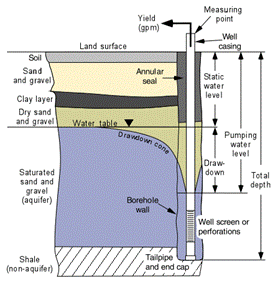
\includegraphics[scale=0.5]{Well1} \hspace{1cm} 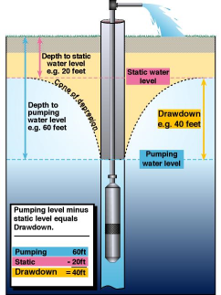
\includegraphics[scale=0.6]{WellDrawdownCalc}
\end{center}

The amount of water a well will produce depends mainly on the type of aquifer, well construction, and the depth of the zone of saturation. The annual recharge rate from percolation, along with the ability of the water bearing formation to transmit water to any given point, will also influence well production. The performance of a well can be determined by taking readings of the hydraulic conditions. An operator must be familiar with these terms and definitions*, in order to accurately troubleshoot problems that may be discovered.\\
\vspace{0.3cm}
\textbf{Static level }is the water level in a well when the pump is not operating.\\
\vspace{0.3cm}
\textbf{Pumping level} is the water level in the well when it is producing.\\
\vspace{0.3cm}
\textbf{Drawdown} is the difference in elevations between the static level and the pumping level. The amount of water produced is approximately proportional to the draw-down. For example, increasing the yield by 10\% will increase the drawdown by 10\%. The draw-down that occurs when a well is running is roughly equal to the head loss encountered in moving the water into the well. Water bearing formations of gravel, limestone and course sand will usually provide more water with less draw-down than formations containing fine sand or clay.\\
\vspace{0.3cm}
\textbf{Specific capacity} is the relationship between the yield of a well and the amount of drawdown in the well. It can be expressed as a ratio of the yield, in terms of gallons per minute, to the drawdown in feet. A well producing 100 gpm with a drawdown of 20 feet would have a specific capacity of 5 gpm per foot of draw-down. In this particular case every time the yield is increased by 5 gpm the drawdown will increase by one foot. This relationship will exist until the yield exceeds the aquifer’s ability to deliver water to any single point, When this limit is reached, the draw-down increases dramatically with little or no increase in the yield.\\
\vspace{0.3cm}
\textbf{Cone of depression} is directly related to the drawdown in the well. As the pump draws down the water level, a portion of the aquifer surrounding the well is drained of water. A cone shaped depression is formed in the water table around the well. The shape of the cone will vary depending on the type of formation in which the well is located. A fine sand formation will usually create a steep cone of depression, while a shallow cone is usually found in coarse sand and gravel formations.\\
\vspace{0.3cm}
\textbf{Radius of influence} is the farthest distance from the well that the cone of depression affects the water table. This distance can be determined by sinking test holes around the well and monitoring the water levels in them while the well is pumping.\\
\vspace{0.3cm}
\textbf{Recovery time} is the amount of time required for the aquifer to stabilize at its static water level once pumping has stopped. This can also be determined by monitoring the water levels in the test holes used to determine the radius of influence.\\


  \vspace{0.3cm}
\textbf{Example Problem \#1:} A well is drilled through an unconfined aquifer. The top of the aquifer is 80 feet below grade. After the well was in service for a year, the water level in the well stabilized at 110 feet below grade. What is the drawdown?\\
$\text {Drawdown} =\text { Static Level}-\text { Pumping Level } =80 \mathrm{ft}-110 \mathrm{ft}=30 \mathrm{feet}$


\textbf{Example Problem \#2:} A well produces 300 gpm. If the drawdown is 30 feet, find the specific yield.\\
$\text { Specific Yield } =\dfrac{\text { Yield }}{\text { Drawdown }} =\dfrac{300 \mathrm{gpm}}{30 \mathrm{ft}} =10 \mathrm{gpm} / \mathrm{ft}$
  \vspace{0.3cm}
\textbf{Example Problem \#3:} The specific yield for a well is $10 \mathrm{gpm} / \mathrm{ft}$. If the well produces $550 \mathrm{gpm}$, what is the drawdown?\\
  \vspace{0.3cm}
$\text {Specific Yield }=\dfrac{\text { Yield }}{\text { Drawdown }}\implies 10 \mathrm{gpm} / \mathrm{ft}=\dfrac{550 \mathrm{gpm}}{\text { Drawdown }}$\\
\vspace{0.3cm}
$\implies \text {Drawdown }= \dfrac{550}{10}=\boxed{55 \mathrm{ft}}$ \\
\vspace{0.3cm}
\textbf{Example Problem \#3:} The pumped water level of a well is 400 feet below the surface. The well produces 350 gpm. If the aquifer level is 250 feet below the surface, what is the specific yield for the well?\\
  $\text {Drawdown} =\text { Static Level}-\text { Pumping Level } =400 \mathrm{ft}-350 \mathrm{ft}=50 \mathrm{feet}$\\
  $\text {Specific Yield }=\dfrac{\text { Yield }}{\text { Drawdown }}=\dfrac{350 \mathrm{gpm}}{\text { 50 }}=7 \mathrm{gpm} / \mathrm{ft}$ \\


\section{Force, Pressure and Head} \index{Force, Pressure and Head}

\textbf{Force:}  In the English system force and weight are often used in the same way. The weight of the cubic foot of water is $62.4$ pounds. The force exerted on the bottom of the one foot cube is $62.4$ pounds. If we have two cubes stacked on top of one another, the force on the bottom will be $124.8$ pounds.

\textbf{Pressure:} Pressure is a force per unit of area, pounds per square inch or pounds per square foot are common expressions of pressure. 

\textbf{Head:}  Pressure is directly related to the height of a column of fluid. This height is called head or feet of head. Pressure and feet of head head are directly related - \emph{for every one foot of head there is a pressure of $0.433$ psi.}

\vspace{0.2cm}
Thus, $\dfrac{0.433 \enspace psi}{ft \enspace (water \enspace column)}$ or conversely $\dfrac{1 \enspace ft \enspace (water \enspace column)}{2.31 \enspace psi}$\\
\texthl{Note:  This pressure/head will include the height the water pumped and also the head associated with friction losses - energy loss because of the water moving through the pipe and fittings.}\\

\begin{figure}[h]
\begin{tikzpicture}
\path[help lines,step=.2] (0,0) grid (16,6);
\path[help lines,line width=.6pt,step=1] (0,0) grid (16,6);
%\foreach \x in {0,1,2,3,4,5,6,7,8,9,10,11,12,13,14,15,16}
%\node[anchor=north] at (\x,0) {\x};
%\foreach \y in {0,1,2,3,4,5,6}
%\node[anchor=east] at (0,\y) {\y};
\pgfmathsetmacro{\cubex}{3}
\pgfmathsetmacro{\cubey}{3}
\pgfmathsetmacro{\cubez}{3}
\draw(13.5,5,3) -- ++(-\cubex,0,0) -- ++(0,-\cubey,0) -- ++(\cubex,0,0) -- cycle;
\draw(13.5,5,3) -- ++(0,0,-\cubez) -- ++(0,-\cubey,0) -- ++(0,0,\cubez) -- cycle;
\draw(13.5,5,3) -- ++(-\cubex,0,0) -- ++(0,0,-\cubez) -- ++(\cubex,0,0) -- cycle;
\draw (8.7,2.5) node[text width=3cm,align=center]
  {\scriptsize{12"}};
\draw (14.1,3.4) node[text width=3cm,align=center]
  {\scriptsize{12"}};
  \draw (10.9,0.5)node[text width=3cm,align=center]
  {\scriptsize{12"}};
    \draw (2.8,4.8)node[text width=3.8cm,align=left]
  {\small{$Pressure=\dfrac{Force}{Area}$}};
      \draw (2.8,3.1)node[text width=3.8cm,align=left]
  {\small{Pressure exerted by}};
        \draw (2.8,2.8)node[text width=3.8cm,align=left]
  {\small{a 1ft column of water}};
        \draw (5.3,2.9)node[text width=3cm,align=center]
  {\small{$=\dfrac{62.4 \enspace lb}{12 in \enspace x \enspace 12 in}$}};
          \draw (7.3,2.9)node[text width=3cm,align=center]
  {\small{$=0.43 \enspace psi$}};
         \draw (3.45,1.2)node[text width=5cm,align=left]
  {\small{As 1$ft^3$ of water weighs 62.4 lbs}};
\end{tikzpicture}
\end{figure}


The pressure at the bottom of a container is affected only by the height of water in the container and not by the shape or the volume of the container. In the drawing below there are four containers all of different shapes and sizes. The pressure at the bottom of each is the same.

\begin{center}
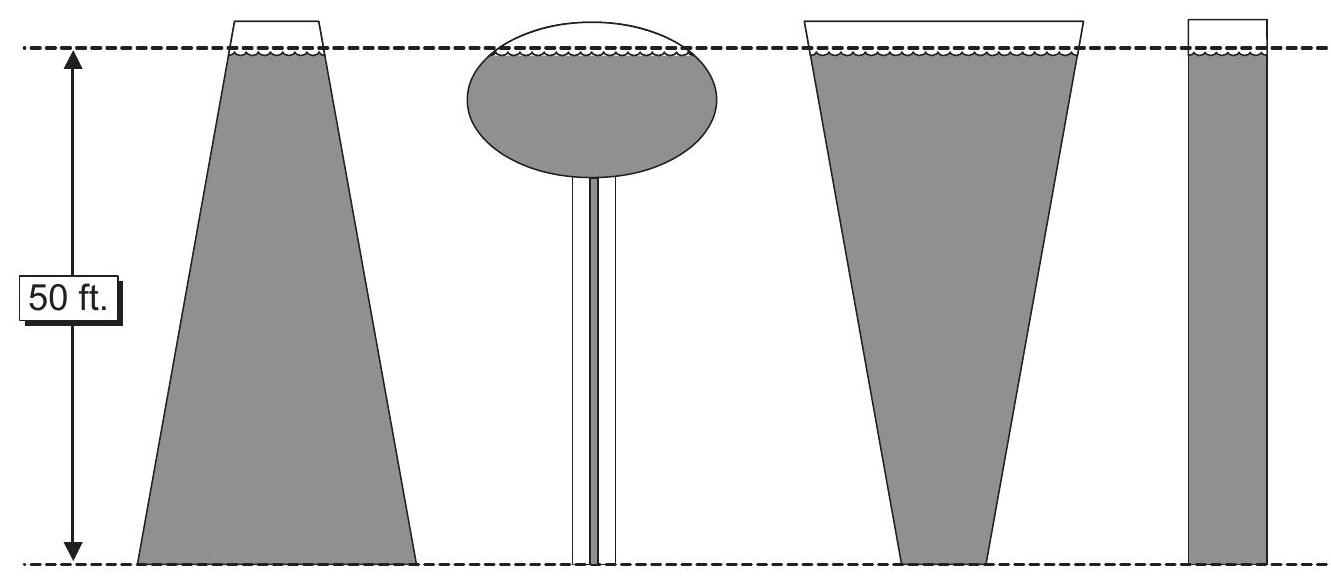
\includegraphics[scale=0.2]{2022_11_03_65aa625ded296bdfd01fg-17}
\end{center}
The pressure exerted at the bottom of a tank is relative only to the head on the tank and not the volume of water in the tank. For example, below are two tanks each containing 5000 gallons. The pressure at the bottom of each is 22 psi. If half of the water were drained from the tanks the pressure at the bottom of the elevated tank would be $17.3$ psi while the pressure at the bottom of the standpipe would be 11 psi.\\

\begin{center}
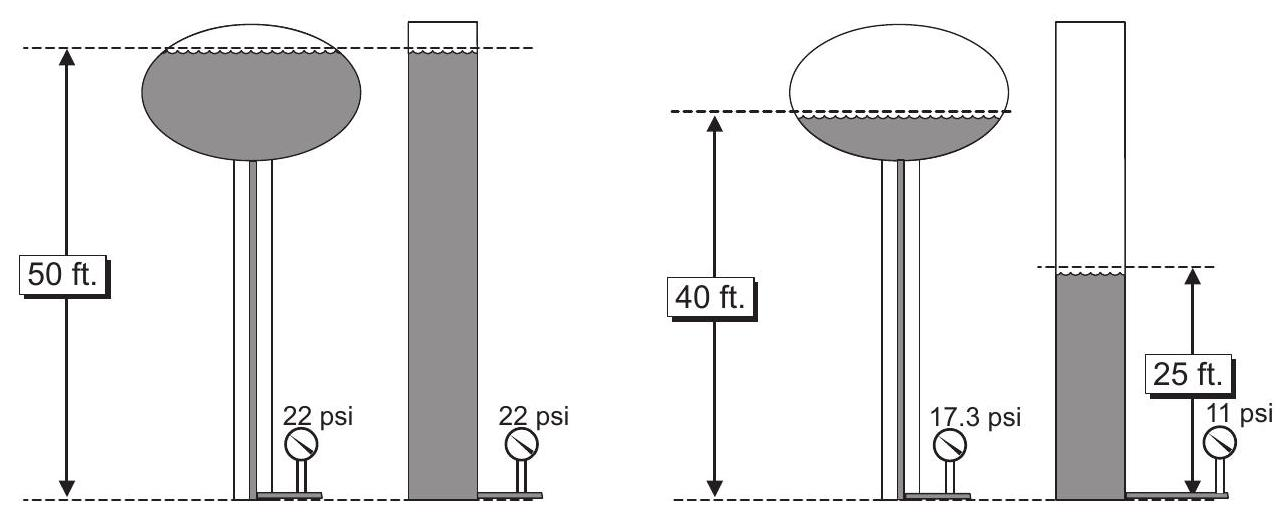
\includegraphics[scale=0.25]{2022_11_03_65aa625ded296bdfd01fg-18}
\end{center}


\begin{itemize}
\item A reservoir is 40 feet tall. Find the pressure at the bottom of the reservoir.

$40 \mathrm{ft} \times 0.433 \mathrm{psi} / \mathrm{ft}=17.3 \mathrm{psi}$

\vspace{0.4cm}

\item Find the height of water in a tank if the pressure at the bottom of the tank is 12 psi.

$12 \mathrm{psi} \div 0.433 \mathrm{psi} / \mathrm{ft}=27.7 \mathrm{ft}$

\vspace{0.4cm}

\item If a pump discharge pressure gauge read 10 psi, the height of the water corresponding to this pressure would be:
$$10 \enspace psi \times \dfrac{2.31 \enspace ft}{psi}=23.1 \enspace ft$$\\
\vspace{0.4cm}
\end{itemize}

\section{Pumping Calculations}\index{Pumping Calculations}
\begin{itemize}
\item Pump is a machine used for moving water (and other fluids) through a piping system and raise the pressure of the water.
\item Pumping is accomplished by transforming the input energy - typically from an electric motor or from other sources such as high-pressure air.
\item The pump calculations in this section are for electrically driven rotodynamic pumps.
\item To move water, a pump will need to overcome resistance due its density, gravitational force and friction.
\item This resistance is dependent on:
\begin{itemize}
\item Height the water needs to be raised.  This height of the fluid in a container is referred to as head. 
\item Quantity of water involved
\end{itemize}
\end{itemize}

\subsection{Glossary of Pump Calculations Terms}\index{Glossary of Pump Calculations Terms}

\textbf{Static Pressure: } Static implies a non-moving condition.  The pressure measured when there is no water moving in a line or the pump is not running is called static $^{32}$ pressure. This is the pressure represented by the gauges on the tanks in the discussion above.

\textbf{Dynamic Pressure: } When water is allowed to run through a pipe and the pressure (called pressure head) measured at various points along the way we find that the pressure decreases the further we are from the sources.
\begin{center}
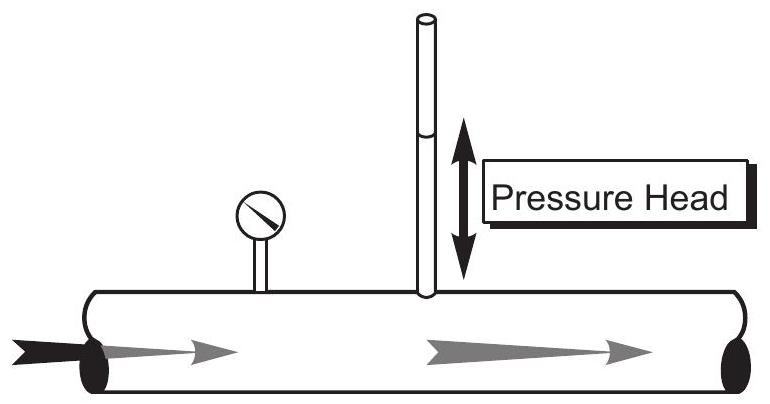
\includegraphics[scale={0.2}]{2022_11_03_65aa625ded296bdfd01fg-18(1)}
\end{center}
\textbf{Headloss: }  The reason for this reduction in pressure is a phenomenon called headloss. Headloss is the loss of energy (pressure) due to friction. The energy is lost as heat.

If the headloss in a certain pipe is 25 feet, it means the amount of energy required to overcome the friction in the pipe is equivalent to the amount of energy that would be required to lift this amount of water straight in the air 25 feet.

In a pipe, the factors that contribute to headloss include the following:

\begin{itemize}
  \item Roughness of pipe - If the roughness of a pipe were doubled the headloss would double.

  \item Length of pipe - If the length of the pipe were doubled the headloss would double.

  \item Diameter of pipe - If the diameter of a pipe were doubled the headloss would be cut in half

  \item Velocity of water - If the velocity of the water in a pipe were doubled the headloss would be increased by about four times. It should be apparent that velocity, more than any other single factor, affects headloss. To double the velocity we would have to double the flow in the line.
  
  \item Pumping System Components and Fittings - Each type of fitting has a specific headloss depending upon the velocity of water through the fitting. For instance the headloss though a check valve is two and one quarter times greater than through a ninety degree elbow and ten times greater than the headloss through an open gate valve.

\end{itemize}

\textbf{Static Head: }  Static head is the distance between the suction and discharge water levels when the pump is shut off. 

\textbf{Suction Lift: } Suction lift is the distance between the suction water level and the center of the pump impeller. This term is only used when the pump is in a suction lift condition. A pump is said to be in a suction lift condition any time the eye (center) of the impeller is above the water being pumped.

\textbf{Velocity Head: } The amount of energy required to bring a fluid from standstill to its velocity. For a given quantity of flow, the velocity head will vary indirectly with the pipe diameter.

\textbf{Total Dynamic Head (TDH):}  The total energy needed to move water from the center line of a pump (eye of the first impeller of a lineshaft turbine) to some given elevation or to develop some given pressure. This includes the static head, velocity head and the headloss due to friction. 

\textbf{Horsepower: } Horsepower is a measurement of the amount of energy required to do work. Motors are rated in horsepower. The horsepower of an electric motor is called brake horsepower. The horsepower requirements of a pump are dependent on the flow and the total dynamic head.  33,000 foot pounds per minute of work is 1 horsepower.

\textbf{Suction Head: } Suction head is the distance between the suction water level and the center of the pump impeller when the pump is in a suction head condition. A pump is said to be in a suction head condition any time the eye (center) of the impeller is below the water level being pumped.

\textbf{Velocity Head: } Velocity head is the amount of energy required by the pump and motor to overcome inertia and bring the water up to speed. Velocity head is often shown mathematically as $\mathrm{V}^{2} / 2 \mathrm{~g}$. ( $\mathrm{g}$ is the acceleration due to gravity $-32.2 \mathrm{ft} / \mathrm{sec}^{2}$ ).
\begin{center}
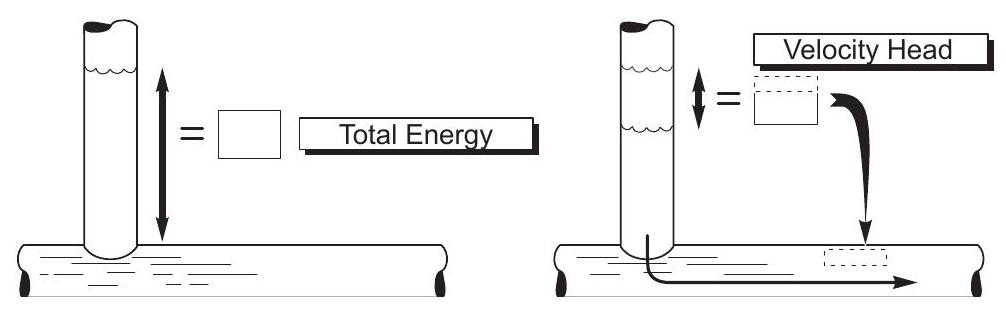
\includegraphics[scale=0.25]{2022_11_03_65aa625ded296bdfd01fg-20}
\end{center}
\textbf{Total Dynamic Head: }  Total dynamic head (TDH) is a theoretical distance. It is the static head, velocity head and headloss required to get the water from one point to another.

The horsepower output of an electric motor is directly reflected to the amperage that the motor draws. Any increase in horsepower requirements will give a corresponding increase in amperage.

\textbf{Cavitation: }  Cavitation in pumps is the rapid creation and subsequent collapse of air bubbles occuring as a result of the inlet pressure falling below the design inlet pressure or when the pump is operating at a flow rate higher than the design flow rate. This collapse of the air bubbles typically manifests as a pinging or crackling noise.  Cavitation is undesirable because it can damage the impeller, cause noise and vibration, and decrease pump efficiency.

\begin{figure}[h]
\begin{center}
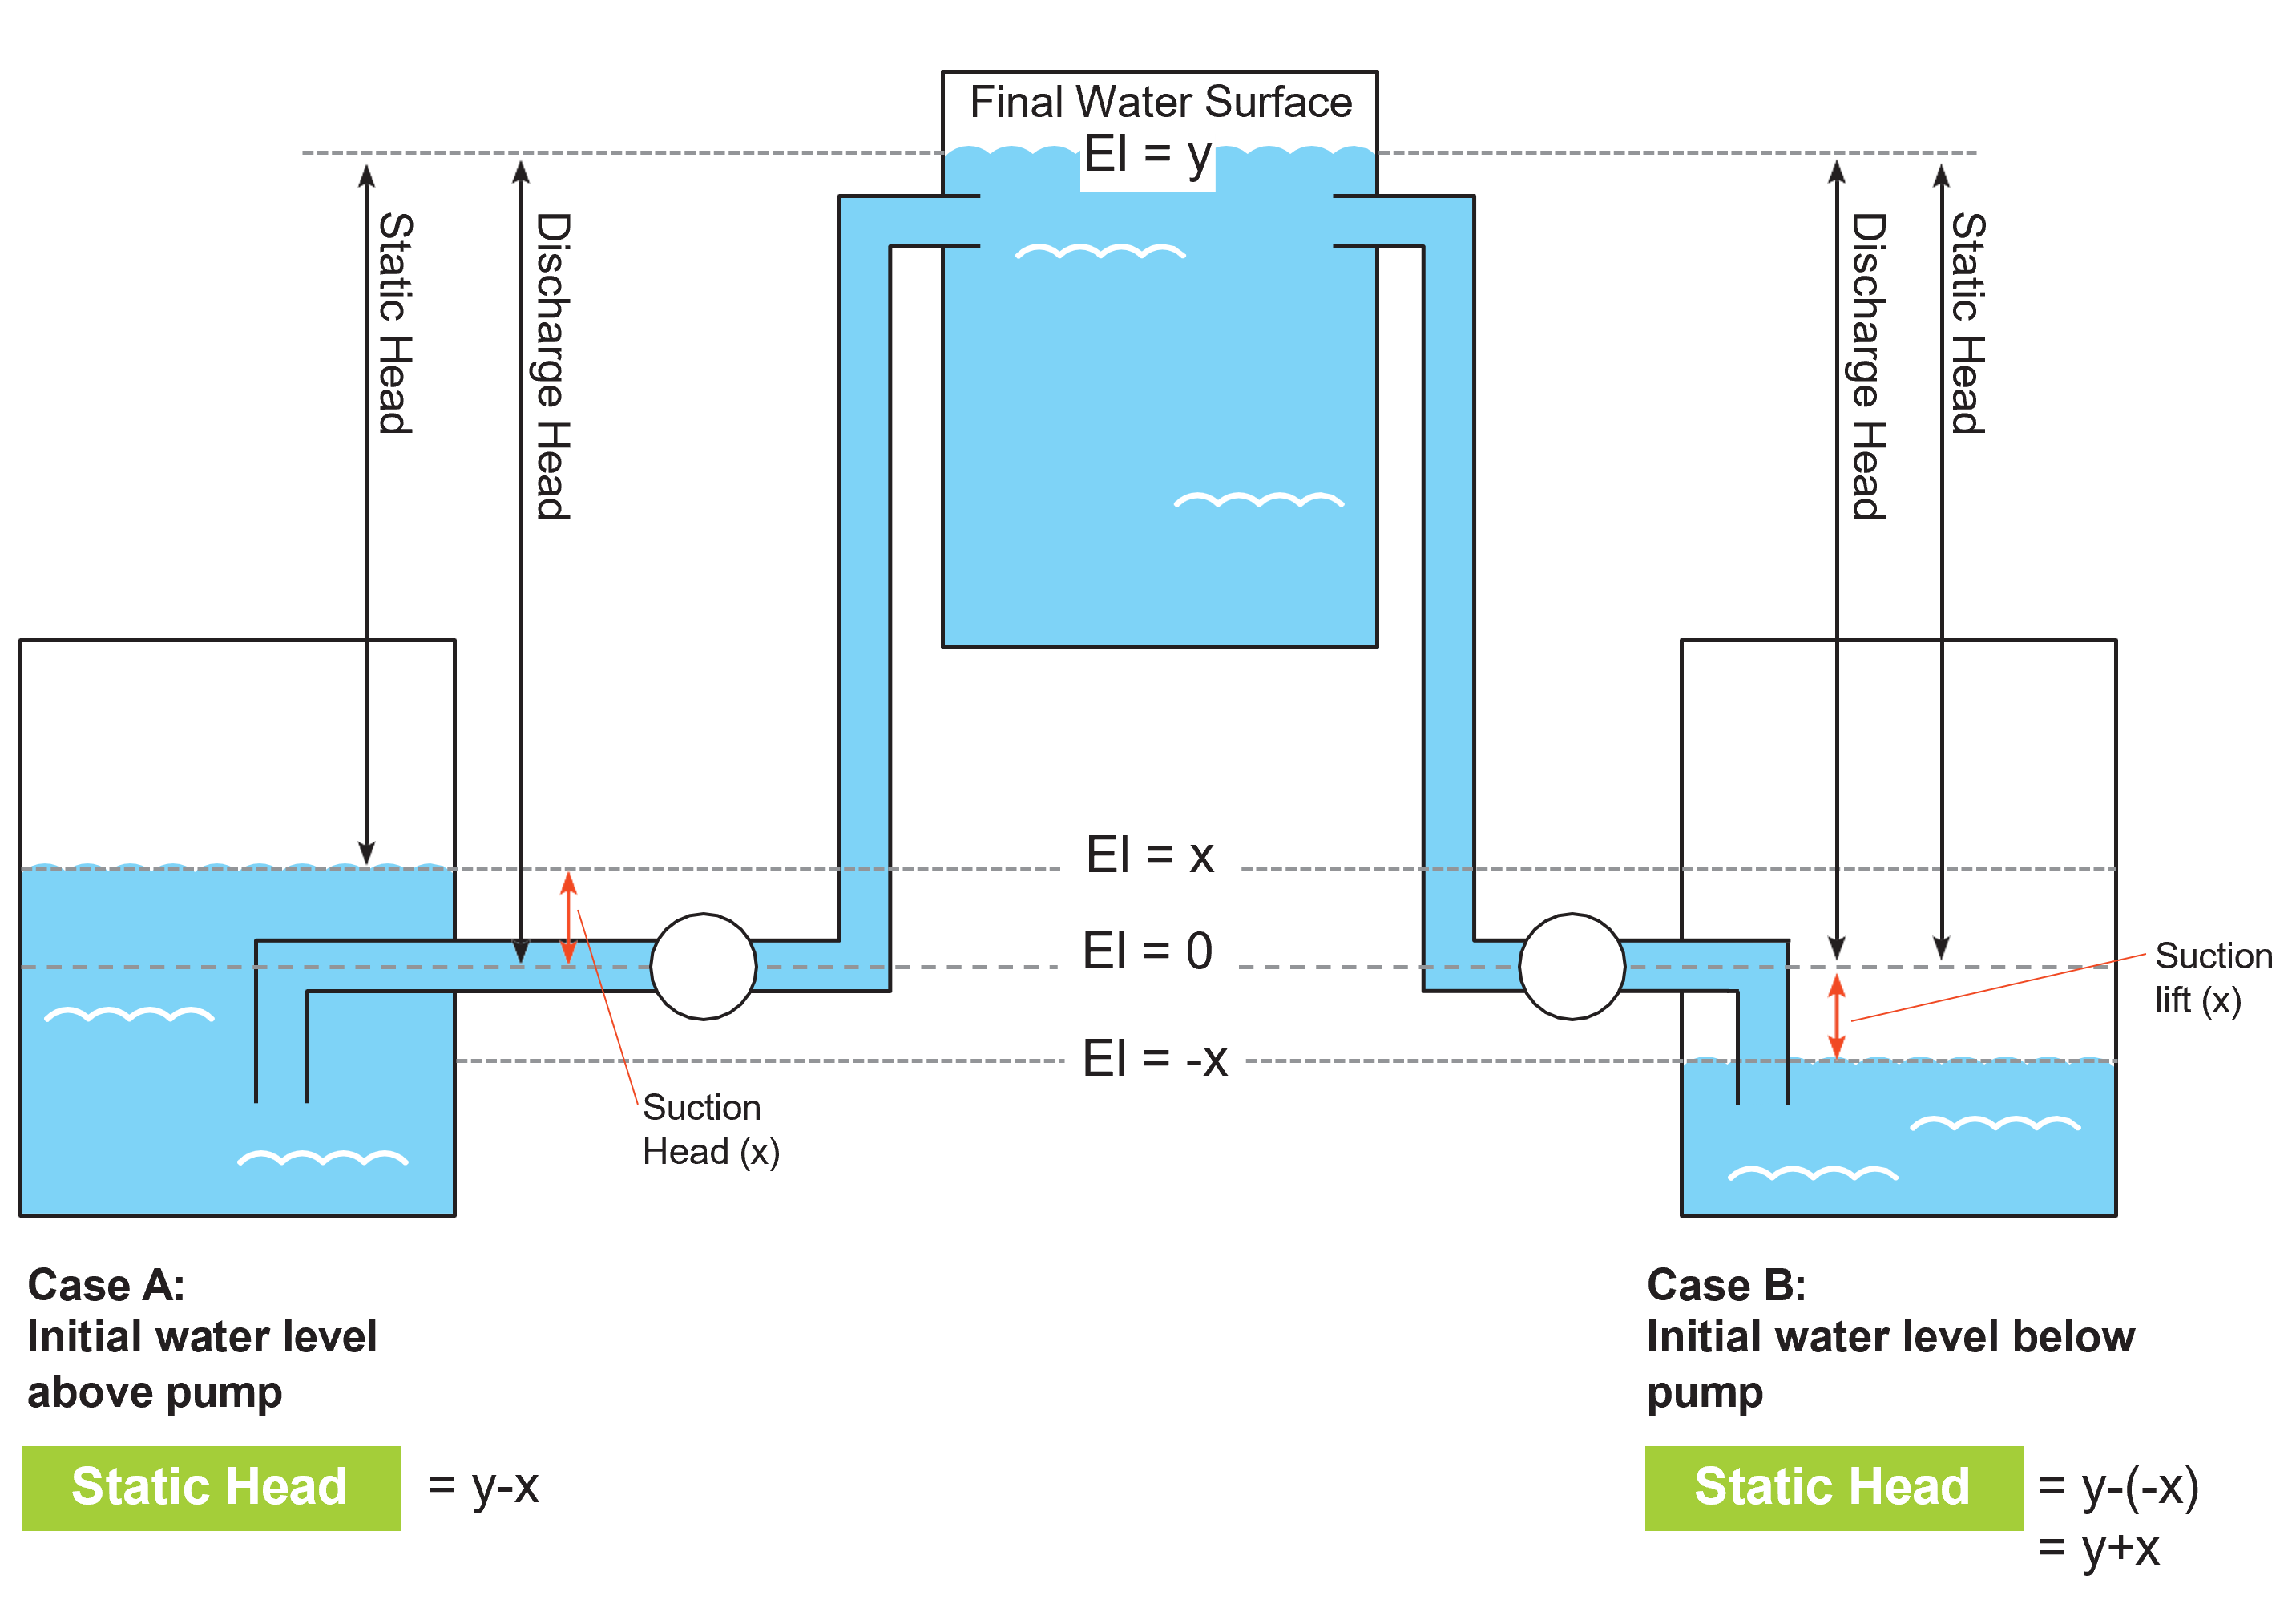
\includegraphics[scale=0.6]{CalculatingStaticHead}\\
\includegraphics[scale=0.6]{PumpHead}\\
\end{center}
\end{figure}

\subsection{Pumping Rate Calculations}\index{Pumping Rate Calculations}
\begin{itemize}
\item \texthl{For calculating volume pumped given the pump flow rate:} Multiply the pump flow rate by the time interval\\
\textbf{Make sure:}
\begin{itemize}
\item The time units - in the given time interval and in the pump flow rate match
\end{itemize}
\item \texthl{For calculating time to pump a certain volume:}
\begin{enumerate}[Step 1.]
\item Calculate the total volume pumped
\item Divide the total volume by the pump flow rate
\end{enumerate}
\textbf{Make sure:}
\begin{itemize}
\item The volume units - in the volume that needs to be pumped and in the pump flow rate match
\item The time unit in the pump flow rate needs to be converted to the time unit that you need the answer in
\end{itemize}
\end{itemize}
% \end{enumerate}

\textbf{Example 1:}  A pump is set to pump 5 minutes each hour. It pumps at the rate of 35 gpm. How many gallons of water are pumped each day?\\
Solution:\\
$\dfrac{35 \enspace gal \enspace sludge}{\cancel{min}}*\dfrac{5 \enspace \cancel{min}}{\cancel{hr}} *\dfrac{24 \enspace \cancel{hr}}{day}=\boxed{\dfrac{4,200 \enspace gallons}{day}}$\\
\vspace{0.5cm}

\textbf{Example 2:}  A pump operates 5 minutes each 15 minute interval.  If the pump capacity is 60 gpm, how many gallons are pumped daily?

$\dfrac{60 \enspace gal \enspace sludge}{\xcancel{min}}*\dfrac{5 \enspace \xcancel{min}}{15 \enspace \cancel{min}}*1440\dfrac{\cancel{min}}{day}=\boxed{\dfrac {28,800 \enspace gal \enspace sludge }{day}}$\\
\vspace{0.5cm}

\textbf{Example 3:}  Given the tank is 10ft wide, 12 ft long and 18 ft deep tank including 2 ft of freeboard when filled to capacity. How much time (minutes) will be required to pump down this tank to a depth of 2 ft when the tank is at maximum capacity using a 600 GPM pump\\
Solution:\\
\vspace{0.5cm}


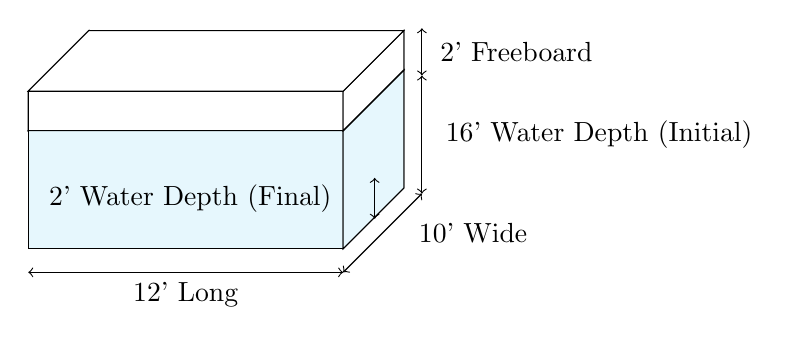
\begin{tikzpicture}

\pgfmathsetmacro{\cubexx}{4}
\pgfmathsetmacro{\cubeyy}{1.5}
\pgfmathsetmacro{\cubezz}{2}
\pgfmathsetmacro{\cubex}{4}
\pgfmathsetmacro{\cubey}{0.5}
\pgfmathsetmacro{\cubez}{2}
\pgfmathsetmacro{\cubexxx}{4}
\pgfmathsetmacro{\cubeyyy}{4}
\filldraw [fill=cyan!10!white, draw=black] (0,-\cubey,0) -- ++(-\cubexx,0,0) -- ++(0,-\cubeyy,0) -- ++(\cubexx,0,0) -- cycle ;
\filldraw [fill=cyan!0!white, draw=black] (0,-\cubey,0) -- ++(0,0,-\cubezz) -- ++(0,-\cubeyy,0) -- ++(0,0,\cubezz) -- cycle;
\filldraw [fill=cyan!10!white, draw=black] (0,-\cubey,0) -- ++(0,0,-\cubezz) -- ++(0,-\cubeyy,0) -- ++(0,0,\cubezz) -- cycle;
%\filldraw [fill=cyan!10!white, draw=black] (0,-\cubey,0) -- ++(-\cubexx,0,0) -- ++(0,0,-\cubezz) -- ++(\cubexx,0,0) -- cycle;
%%%\draw (0,-0.5,0) -- ++(-\cubex,0,0) -- ++(0,-\cubey,-\cubez) -- ++(\cubex,0,0) -- cycle;
\draw (-\cubex,0,0) -- ++(0,0,-\cubez) -- ++(0,-\cubey,0) -- ++(0,0,\cubez) -- cycle;
\draw (0,-\cubey,0) -- ++(-\cubex,0,0) -- ++(0,0,-\cubez) -- ++(\cubex,0,0) -- cycle;
\filldraw [fill=white, draw=black] (0,0,0) -- ++(-\cubex,0,0) -- ++(0,-\cubey,0) -- ++(\cubex,0,0) -- cycle ;
\filldraw [fill=white, draw=black] (0,0,0) -- ++(0,0,-\cubez) -- ++(0,-\cubey,0) -- ++(0,0,\cubez) -- cycle;
\filldraw [fill=white, draw=black] (0,0,0) -- ++(0,0,-\cubez) -- ++(0,-\cubey,0) -- ++(0,0,\cubez) -- cycle;
\filldraw [fill=white, draw=black] (0,0,0) -- ++(-\cubex,0,0) -- ++(0,0,-\cubez) -- ++(\cubex,0,0) -- cycle;

%\filldraw [fill=RoyalBlue!10!white, draw=black] (0,-1.5,0) -- ++(-\cubex,0,0) -- ++(0,-\cubey,0) -- ++(\cubex,0,0) -- cycle ;

%\filldraw [fill=RoyalBlue!10!white, draw=black] (0,-1.5,0) -- ++(0,0,-\cubez) -- ++(0,-\cubey,0) -- ++(0,0,\cubez) -- cycle;



%%\draw (0,-0.5,0) -- ++(-\cubex,0,0) -- ++(0,0,-\cubez) -- ++(\cubex,0,0) -- cycle;
%%\filldraw [fill=white, draw=black] (-\cubex,0,0) -- ++(0,0,-\cubez) -- ++(0,-\cubey,0) -- ++(0,0,\cubez) -- cycle;
%%\filldraw [fill=white, draw=black] (0,-\cubey,0) -- ++(-\cubex,0,0) -- ++(0,0,-\cubez) -- ++(\cubex,0,0) -- cycle ;

\draw [<->] (-4,-2.3) -- (0,-2.3) node [midway, below] {12' Long};
\draw [<->] (1,-1.3) -- (1,.2) node [midway, midway] {\hspace{4.5cm}16' Water Depth (Initial)};
\draw [<->] (0.4,-1.62) -- (0.4,-1.1) node [midway, midway] {\hspace{-4.8cm} 2' Water Depth (Final)};
\draw [<->] (1,.8) -- (1,.2) node [midway, midway] {\hspace{2.4cm}2' Freeboard};
\draw [<->] (1,-1.3) -- (0,-2.3) node [midway, midway] {\hspace{2.3cm}10' Wide};
\end{tikzpicture}\\
Volume to be pumped=$12 \enspace ft*10 \enspace ft *(16-2)\enspace ft=1,680ft^3$\\
\vspace{0.3cm}
$\implies \dfrac{1,680\cancel{ft^3}*7.48\dfrac{\cancel{gal}}{\cancel{ft^3}}}{600\dfrac{\cancel{gal}}{min}}=\boxed{21min}$



\subsection{Power Requirements for Pumping}\index{Power Requirements for Pumping}
\begin{center}
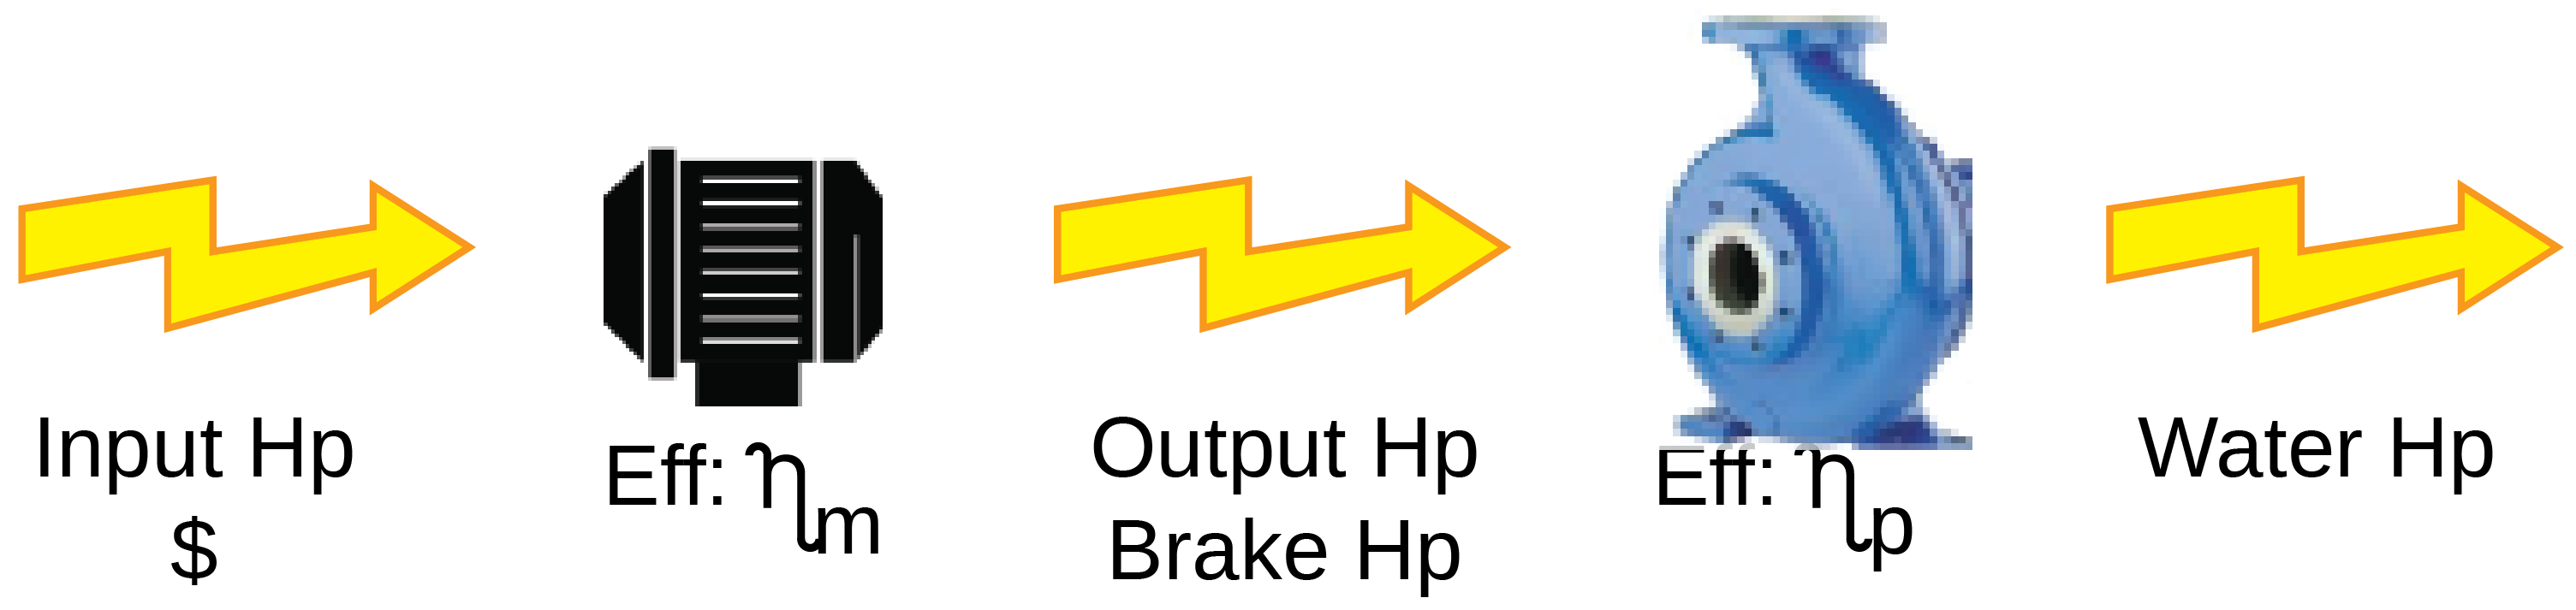
\includegraphics[scale=0.12]{PumpProblem}\\
\end{center}
Where:\\
\begin{itemize}
\item \textbf{Input Hp} is the input power to the motor which produces the \textbf{Output Hp or Brake Hp} - the mechanical power which runs the pump.  
\item The ratio of Output Hp and Input Hp is the motor efficiency - $\eta_m$.
\item The Output Hp is the input power (Brake Hp) to the pump to pump the water.
\item Water Hp is the rate of energy transferred to the water being pumped and can be calculated by the formula:\\
$$\dfrac{\mathrm{H \enspace - \enspace Head \enspace of \enspace water \enspace (ft) \enspace * \enspace Q \enspace - \enspace Flow \enspace (GPM)}}{3,960 \enspace \mathrm{(Conversion \enspace factor \enspace for \enspace converting \enspace GPM-ft \enspace to \enspace Hp)}}$$
\item The ratio of Output Hp and Water Hp is the pump efficiency - $\eta_p$.
\end{itemize}
\subsection{Example Problems}
\begin{enumerate}


\item 1 MGD is pumped against a 14’ head.  What is the water Hp?  The pump mechanical efficiency is 85\%.  What is the brake horsepower?\\
\vspace{0.4cm}
water Hp = flow * head\\
\vspace{0.4cm}
$\dfrac{1,000,000 \enspace gal}{day}*\dfrac{day}{1440 \enspace min}*14 \enspace ft*\dfrac{Hp}{3,960 \enspace GPM-ft}=\boxed{Water \enspace Hp = 2.46 \enspace Hp}$\\
\vspace{0.4cm}
pump Hp = brake Hp * pump efficiency\\
\vspace{0.4cm}
$Brake \enspace Hp = \dfrac{2.46}{0.85}=\boxed{Brake \enspace Hp=2.89Hp}$\\
\vspace{0.4cm}

\item A flow of 200 gpm  is pumped against a total head of 4.0 feet. The pump is 78\% efficient and the motor' is 90\% efficient. Calculate the input Hp.\\
\vspace{0.4cm}
water Hp = flow * head\\
\vspace{0.2cm}
$200GPM*4ft*\dfrac{Hp}{3,960 GPM-ft}=0.2Hp$\\
\vspace{0.4cm}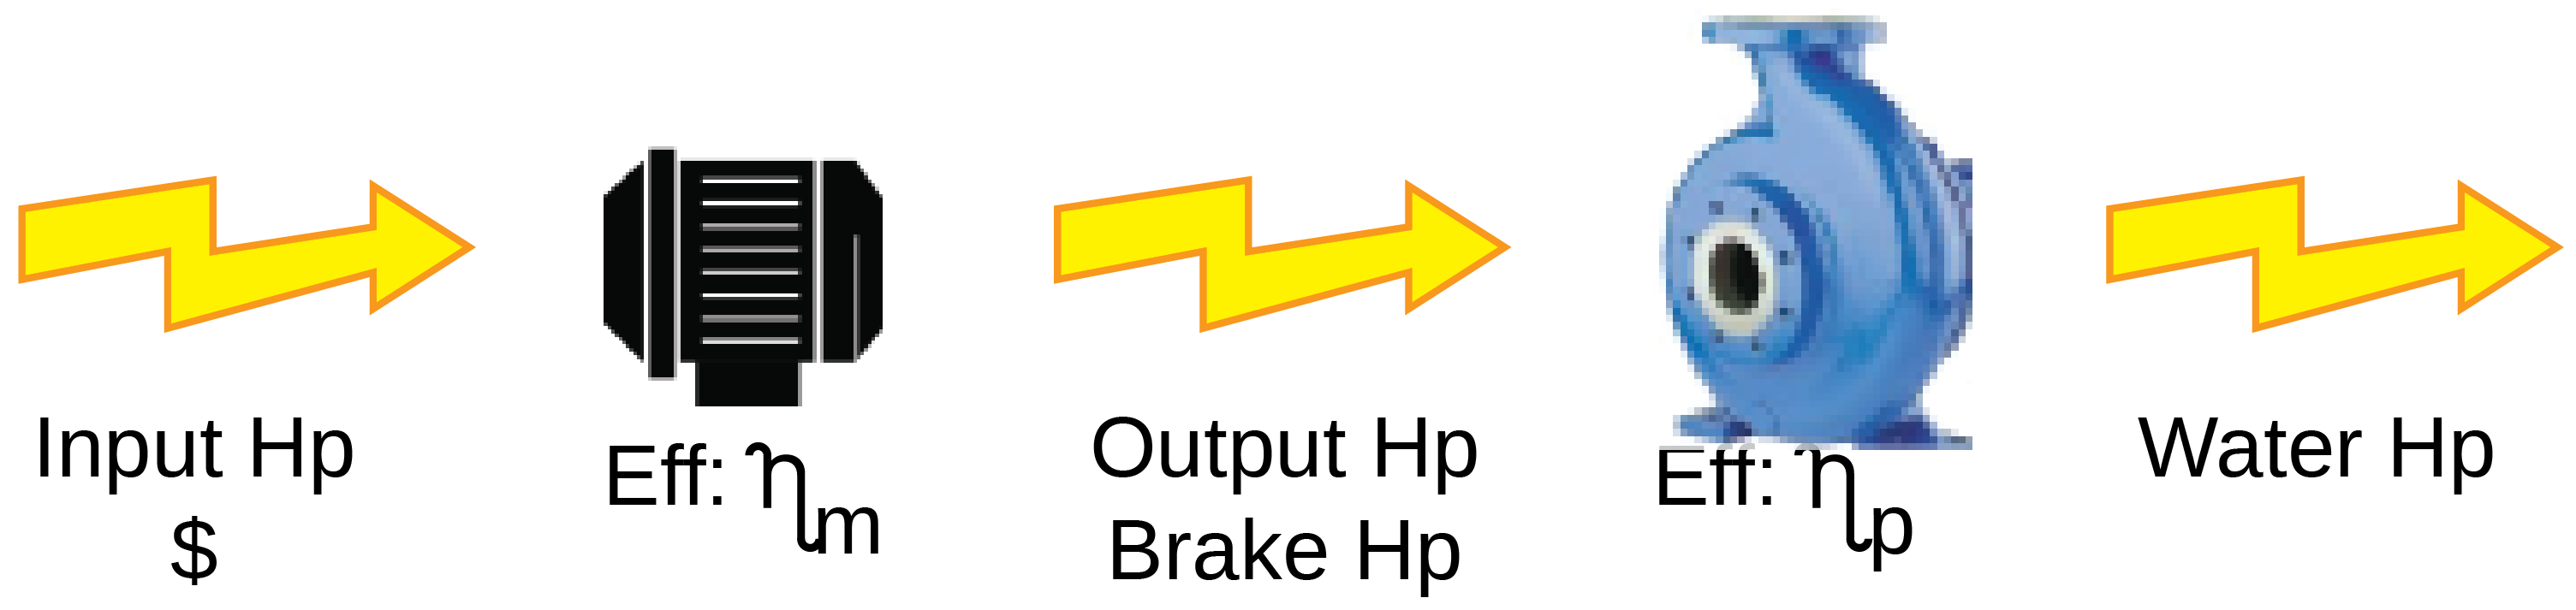
\includegraphics[scale=0.08]{PumpProblem}\\
water Hp=brake Hp*pump efficiency, and\\
brake Hp=input Hp*motor efficiency\\
Therefore, water Hp=input Hp*motor efficiency*pump efficiency\\
\vspace{0.4cm}
input Hp=$\dfrac{water \enspace Hp}{motor \enspace efficiency*pump \enspace efficiency}=\dfrac{0.2}{0.9*0.78}=\boxed{0.28Hp}$
\vspace{0.2cm}
\end{enumerate}


\section{Detention Time}\index{Detention Time}
\begin{itemize}
\item \colorbox{lime}{Detention Time} - The actual or theoretical (calculated) time required for water to fill a tank at a given flow; pass through a tank at a given flow; or remain in a settling basin, flocculating basin, rapid-mix chamber, or storage tank.\\
$$Tank/clarifier \enspace detention \enspace time \enspace (hr) = 	\dfrac{ Tank/clarifier \enspace volume (cu.ft \enspace or \enspace gal)}{Influent \enspace flow \enspace (cu.ft \enspace or \enspace gal)/hr)}$$
Rectangular tank/clarifier volume = width * length * depth of water\\
Circular tank/clarifier volume = 0.785 * Diameter$^2$ * depth of water\\
Typically volume is calculated in cu. ft and influent flow is given in gallons.  Use 7.48 gal/ft$^3$ conversion factor to convert volume in cu. ft to gallons.\\
\end{itemize}

\section{Sedimentation}\index{Sedimentation}
\begin{enumerate}
\item \colorbox{lime}{Hydraulic or Surface Loading Rate} - measures how rapidly wastewater moves through the sedimentation tank or clarifier.  It is measured in terms of the number of gallons flowing each day through one square foot surface area of the clarifier.

The hydraulic or surface loading rate  
$$Clarifier \enspace hydraulic \enspace loading \enspace 	\Big(\dfrac{gpd}{ft^2}\Big) =\dfrac{Clarifier \enspace influent 	\enspace flow (gpd)}{Clarifier \enspace surface \enspace area 	(ft^2)}$$ 
		Rectangular clarifier surface area  = width * length\\
		Circular clarifier surface area  = 0.785 * Diameter$^2 $\\
\item \colorbox{lime}{Detention Time} - it is the length of time that water stays in the sedimentation tank.  It is also the time it takes for a unit volume of water to pass entirely through it.\\
$$Clarifier \enspace detention \enspace time \enspace (hr) = 	\dfrac{ Clarifier \enspace volume (cu.ft \enspace or \enspace gal)}{Influent \enspace flow \enspace (cu.ft \enspace or \enspace gal)/hr)}$$
Rectangular clarifier volume = width * length * depth of water\\
Circular clarifier volume = 0.785 * Diameter$^2$ * depth of water\\
Typically volume is calculated in cu. ft and influent flow is given in gallons.  Use 7.48 gal/ft$^3$ conversion factor to convert volume in cu. ft to gallons.\\

\item \colorbox{lime}{Overflow Rate} - The weirs at the end of the sedimentation basin allow for the even distribution of the the outlet flow across the entire length of the weir.  An adequate length of weir is needed to ensure smooth and even flow of water over the weirs.  Weir overflow rate measures the number of gallons of water per day flowing over one foot of weir. 

		$$Weir \enspace over \enspace flow \enspace rate \Big(\dfrac{gpd}{ft}\Big) =\Big(\dfrac{Clarifier \enspace influent \enspace  flow (gpd)}{Total \enspace effluent 					\enspace weir \enspace length \enspace (ft)}\Big)$$
		Circular clarifier weir length = 3.14 * Diameter\\

Example problem for (a), (b) and (c) above:\\
		\vspace{0.2cm}
A circular clarifier receives a flow of 5 MGD.  If the clarifier is 90 ft. in diameter and is 12 ft. deep, what is: a) the hydraulic/surface loading rate, b) clarifier detention time in hours, and c) weir overflow rate?\\
		\vspace{0.2cm}
a) Hydraulic/surface loading rate:\\
$Clarifier \enspace hydraulic \enspace loading \enspace 	\Big(\dfrac{gpd}{ft^2}\Big) ==\dfrac{\dfrac{5\cancel{MG}}{{day}}*\dfrac{10^6gal}{\cancel{MG}}}{0.785*90^2 ft^2}=\boxed{786gpd/ft^2}$\\
		\vspace{0.5cm}
b) Clarifier detention time:\\
$Clarifier \enspace detention \enspace time \enspace (hr) = 	\dfrac{ Clarifier \enspace volume (cu.ft \enspace or \enspace gal)}{Influent \enspace flow \enspace (cu.ft \enspace or \enspace gal)/hr)}$\\
		\vspace{0.2cm}
$Clarifier \enspace detention \enspace time \enspace (hr) = 	\dfrac{(0.785*90^2*12)\cancel{ft^3}}{\dfrac{5\cancel{MG}}{\cancel{day}}*\dfrac{10^6\cancel{gal}}{\cancel{MG}}*\dfrac{\cancel{ft^3}}{7.48\cancel{gal}}*\dfrac{\cancel{day}}{24hrs}}=\boxed{2.7hrs}$\\
		\vspace{0.5cm}
c) Overflow rate:\\
		\vspace{0.2cm} 
$Weir \enspace overflow \enspace rate \Big(\dfrac{gpd}{ft}\Big) =\dfrac{\dfrac{5\cancel{MG}}{{day}}*\dfrac{10^6gal}{\cancel{MG}}}{3.14*90 ft}=\boxed{17,692 \mathrm{gpd}/\mathrm{ft}}$\\
\end{enumerate}


\section{Filtration}\index{Filtration}
Filtration process typically involves following types of calculations:
\begin{enumerate}
\item \colorbox{lime}{Filter Flow Rates} – the flow rate expressed in gpm can be calculated from the total flow over certain time or vice-versa can be used for determining either the time it would take to process a certain flow or calculate the total flow.\\

 

 

\textbf{Example Problem:}  A filter box is 20 ft by 30 ft (including the sand area). If the influent valve is shut, the water drops 3 inches per minute. What is the rate of filtration in MGD?\\

\vspace{0.3cm}
Filter flow rate=$\Big((20 \enspace \mathrm{ft} \times 30 ft)ft^2* \dfrac{3 \enspace \mathrm{in}}{\mathrm{min}}*\dfrac{\mathrm{ft}}{12 \enspace \mathrm{in}}\Big)\mathrm{ft^3}*\dfrac{7.48 \enspace \mathrm{gal}}{\mathrm{ft}^3}=\boxed{1,122 \enspace \mathrm{gpm}} $



\item \colorbox{lime}{Filtration Rates} – It is the gallons of water filtered per minute through each square foot of filter area.  It generally ranging from 2 to $10 \mathrm{gpm} / \mathrm{ft}^{2}$.\\

Filtration rate is determined by the following equation:\\
$$
\text { Filtration rate, } \mathrm{gpm} / \mathrm{ft}^{2}=\dfrac{\text { Flow rate, } \mathrm{gpm}}{\text { Filter surface area, } \mathrm{ft}^{2}}
$$\\

\textbf{Example Problem:} A filter $28 \mathrm{ft}$ long by $18 \mathrm{ft}$ wide treats a flow of $3.5 \mathrm{MGD}$. What is the filtration rate in gpm/ft ${ }^{2}$ ?\\

\vspace{0.2cm}
\textit{Approach:  The flow will need to be converted to gpm and the surface area calculated in feet.}\\

$\text{Filtration rate, } \mathrm{gpm} / \mathrm{ft}^{2} = 
\dfrac{
\dfrac{3.5 \enspace \cancel{MG}}{ \cancel{day}} * \dfrac{1,000,000 \enspace gal}{\cancel{MG}}
*\dfrac{\cancel{day}}{1440 \mathrm{ min}}}
{28 \enspace ft * 18 \enspace feet}= \boxed{4.8 \enspace gpm/ft^2}$\\
\vspace{0.2cm}


\item \colorbox{lime}{Backwashing Rates} - is the amount of water, in gallons, required for each backwash. This is analogous to the Filter Flow Rate.

\textbf{Example Problem:}
A filter has the following dimensions: $30 \mathrm{ft}$ long by $20 \mathrm{ft}$ wide with a depth of 24 inches of filter media. Assuming that a backwash rate of $15 \mathrm{gal} / \mathrm{ft}^{2} / \mathrm{min}$ is recommended and 10 minutes of backwash is required, calculate the amount of water, in gallons, required for each backwash.

\textit{The backwashing rate given in $gal/ft^2/min$ will need to be converted into gallons by multiplying it with the area (to eliminate $ft^2$ and by the backwash time in minutes}

$ \text{Backwashing rate (gal)} = 15\dfrac{gal}{\cancel{ft^2}-\cancel{min}}*(30 \mathrm{ ft} \times 20 \mathrm{ ft})\cancel{ft^2}*10 \enspace \cancel{min}=\boxed{90,000 \enspace \text{gal}}$

\item \colorbox{lime}{Backwash Rinse Rates} - it is the upward velocity of the water during backwashing, expressed as in/min rise. To convert from $\mathrm{gpm} / \mathrm{ft}^{2}$ backwash rate to an in/min rise rate, use either of the following equations:

$$\text{ Backwash rinse rate, in/} \mathrm{min}=\dfrac{\text { Backwash rate, } \mathrm{gpm} / \mathrm{ft}^{2} \times 12 \mathrm{in} / \mathrm{ft}}{7.48 \mathrm{gal} / \mathrm{ft}^{3}}$$

\textbf{Example Problem}
A filter $22 \mathrm{ft}$ long by $12 \mathrm{ft}$ wide has a backwash rate of $3260 \mathrm{gpm}$. What is this backwash rate expressed as a in/min rise?

$$\text{ Backwash rinse rate, in/} \mathrm{min}=\dfrac{\text { Backwash rate, } \mathrm{gpm} / \mathrm{ft}^{2} \times 12 \mathrm{in} / \mathrm{ft}}{7.48 \mathrm{gal} / \mathrm{ft}^{3}}$$

\textit{Based upon the above formula, the Backwash tate in $gpm/ft^2$ needs to be calculated by dividing the gpm flow by the surface area}

$\text{Backwash Rinse Rate, in/} \mathrm{min}=\dfrac{
\Biggl(\dfrac{3260 \mathrm{gpm}}{22 \mathrm{ft} \times 12 \mathrm{ft}}\Biggr) \mathrm{gpm} / \mathrm{ft}^{2} \times 12 \mathrm{in} / \mathrm{ft}
}
{
7.48 \mathrm{gal} / \mathrm{ft}^{3}
}=\boxed{19.7in/min}$


\item \colorbox{lime}{Percent Product Water Used for Backwashing} - the equation for percent of product water used for backwashing calculations used is:\\
$$
\text { Backwash water, } \%=\dfrac{\text { Backwash water, gal }}{\text { Water filtered, gal }} \times 100
$$

\textbf{Example Problem}
A total of $11,400,000$ gal of water was filtered during a filter run. If backwashing used 48,500 gal of this product water, what percent of the product water is used for backwashing?

Backwash water, $\%=\dfrac{48,500 \text { gal }}{11,400,000 \text { gal }} \times 100 = \boxed{0.43 \%}$

\end{enumerate}

